\chapter{The "Stealth" Mission: "Observation"}

\begin{wrapfigure}{O}{\figwidth}
	\begin{center}
		
\includegraphics[width=\figwidth]{pics/17/1.png}
	\end{center}
\end{wrapfigure}
"This is complete bullshit!"  Tink's inherently whiny voice rang through the barracks, triggering exasperated groans from its other occupants. 
"It's the mindless, reactionary vilification of anything new by a bunch of narrow minded, overzealous, tech-illiterates who wouldn't recognize scientific progress if it bit them in their paranoid asses."

Nubby's head poked out of the large crate he was rummaging through. 
"I dunno, if dis Scientific Progress stuff is actually goin aroun' bitin' people, dey might 'ave a point..."

Across the room, Twitch leaned out from the behind the blast shield that separated his workshop from the rest of the room. 
"What if it's something that's supposed to bite people? 
Like a cyber-mastiff or a wallet?"

Nubby tilted his head to the side and scratched one of his boils as he pondered this. 
"I don' fink wallets are supposed ta bite people Twitch."

"Mine does, remember that one time when you tried to pick-"

"I wasn' tryin ta do nuffin! 
I was jus' lookin fer my keys-"

"In MY pockets?"

"Well I'd already checked all mine!"

The two troopers' argument was brought to halt as Tink, tired of being ignored, ran between them and started shouting. 
"SHUT UP SHUT UP SHUT UP! 
This is serious! 
They're going to make us leave EVERYTHING! 
Look!" Tink shoved the data-slate he was holding under Nubby's nose.

Nubby, his face screwed up with effort, began running a finger along the line of text Tink indicated. 
"...team's gear not ta include any arm-a-men' or de-vices of a non-'deptus Mechamani-, err Mechacapus, err Cogboy approved ori-gin…" Nubby looked up at Tink in confusion "Da 'ell does all dat mean?" 

"It means," replied the techie "no pulse carbines, no plasma-gun, and NO SPOT!" 

\begin{wrapfigure}{O}{\figwidth}
	\begin{center}
		
\includegraphics[width=\figwidth]{pics/17/2.png}
	\end{center}
\end{wrapfigure}
"WHAT! 
Let me see that!" the dataslate was abruptly ripped from Tink's hands by Twitch, who began scanning at a far faster pace. 
"Oh shit shit shit shit shit shit, there's more." All three troopers bent over the dataslate. 
"No more than twenty kilograms of Munitorum Grade-B explosives?"

"Do you even have any Munitorum-issue 'splosives left?" asked Nubby. 
Twitch just shook his head and held up the cluster of lasgun power packs he'd been taping together. 
"Oh well, don' worry, I'm sure I can work somefin out if we can get to a depot... 
" Nubby paused as Tink and Twitch both pointed at the last line on the dataslate. 
"No items considered contraband under Administratium edict G-somefin-somefin-stroke-17e, Commissarial decree number… Cogboys… Arbites... 
'Quisition... 
ECCLESIARCHY? 
What does da 'clesiarchy gotta do wif what I can or can' bring on a mission? 
Dis is mental! 
Who's making these rules?"

Tink straightened up and tried to recapture his initial indignant tone. 
"These are direct orders from Inquisitor Sciscitat."

"Wasn' ee da one who got squished by da bug? 
Ee get better or somefin?"

"No, the other Inquisitor the one from the stasis cell. 
He's taking command."

"What? 
Dat pillock? 
Does Sarge know about this?"

"He's in on it! 
They're both down in one of the conference rooms with the diplomacy Adept planning some sort of suicide mission!"

There was a pause while this sank in, followed by Nubby swearing and Twitch abruptly shouting "IT'S HAPPENING! 
I KNEW IT!", and sprinting out of the room.

\begin{wrapfigure}{O}{\figwidth}
	\begin{center}
		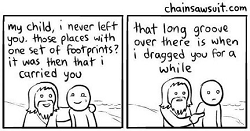
\includegraphics[width=\figwidth]{pics/17/3.png}
	\end{center}
\end{wrapfigure}
Nubby watched the demolitions trooper go, then turned to Tink and asked "So, uh, ou' of curiosity, 'ow exactly did you get dis 'ere list?"

Tink brushed the question aside. 
"That's not important, what is important is that we get together and make it clear to Sarge that we're not going to have any part in this. 
We've got to stand up and say NO, we're not going to go off on a mission without proper equipment." Nubby, his self preservation instincts kicking in, took a step backwards, Tink failed to notice. 
"We're not going to get ourselves killed on some horrible backwater just because of some Inquisitor's ridiculous prejudices.

"Uhhhh, we're not?" Nubby took another step backwards.

"No, we're going to march in there and tell Sarge that either he gets rid of these ridiculous rules, or he goes on his mission alo-URK!" Tink let out a strangled little yelp as a large hand landed on his collar and yanked him backwards.

Somewhere behind Tink, a very deep and angry voice growled, "Guardsman, a word please."

Nubby watched Sarge drag Tink out of room, and let out a sigh of relief as the door slid shut. 
After a few seconds of standing around, listening to muffled shouting and thumping sounds coming through the door, he decided it was probably a good idea to figure out where Twitch went, and possibly join him.

\begin{wrapfigure}{O}{\figwidth}
	\begin{center}
		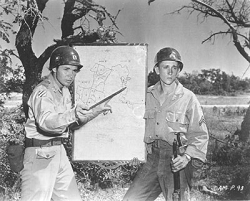
\includegraphics[width=\figwidth]{pics/17/4.png}
	\end{center}
\end{wrapfigure}

\greentext{>Sarge's Rules About What You Can and Can't Bring on a "Stealth" Mission With Inquisitor Asshat}


No Pulse Weapons
Because people notice when lasguns fire little blue balls of plasma, that's why
No Tink's techno-heretical plasma monstrosity
No Spot
Not even if you make him a REALLY GOOD DISGUISE
Nothing, no matter how small, easy to hide, or "awesome", which could be described with the prefix XENO
No, we are NOT bringing Fio. 
Why would you even ask that?
No more than 20 kg of Munitorum-issue explosives
No piles of ammunition for weapons we don't use
Nothing that is almost but not-quite an explosive
Nothing that came out of Sergeant Gravis
NO CHEMICAL, BIOLOGICAL, OR WARP-BASED WEAPONS PERIOD
No contraband
If you have to ask, it's contraband
Your bags will be checked Nubby
No Fumbles or Aimy
Just because Fumbles can turn invisible sometimes does not mean he's stealthy
Medical patients regrowing their entire scalp are not stealthy either
No Jim, Hannah, or Sister Valerie
Because they're staying on the Occurrence Border
No Occurrence Border
BECAUSE A SPACE HULK IS THE OPPOSITE OF STEALTHY, THAT'S WHY
No detailed plans to kill the Inquisitor, desert, and enlist in the Kulthian Foreign Legion
Because the Emperor hates you, that's why

\greentext{>The All Guardsmen Party and Inquisitor Asshat's Stupid "Stealth" Mission}


\begin{wrapfigure}{O}{\figwidth}
	\begin{center}
		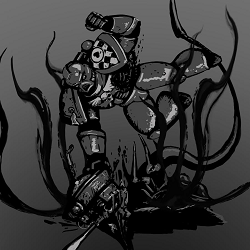
\includegraphics[width=\figwidth]{pics/17/5.png}
	\end{center}
\end{wrapfigure}
So, no shit, we'd finally delivered the requested Zoanthrope. 
It'd taken the crippling, marooning, and deaths of two squads of Space Marines, gratuitous use of heretical xenotech, an assault on a technically-friendly civilian space station, the second worst worst warp voyage in the history of the Imperium, our arrest on trumped up charges by a traitorous Inquisitor, yet another pitched battle when said Inquisitor tried to steal the Zoanthrope for his private collection, and the general maiming of yet another squad of Marines, but we'd FINALLY delivered it. 


Admittedly the bug had suffered some wear and tear during transit; 
what with the theoretically-impossible Daemonic possession, and the way it'd been beaten to the very edge of death by a humorously shaped piece of wraithbone wielded by enraged Space Marine. 
But nowhere in our orders did it say that the thing had to be in good condition. 
It was Zoanthrope, it was alive (if only barely), and only the most ungrateful, pedantic, asshole would dare complain about the quality of the package after the sheer hell we'd been through to deliver it…

Of course "ungrateful", "pedantic", and "asshole" were just about the perfect words to describe Inquisitor Sciscitat, and if you added "bat-shit insane" it'd cover the Magos that ran the research facility as well.

The first thing the two of them did after the Inquisitor had been released from stasis was hold a meeting with us, the Diplomacy Adept, and a few their own minions. 
Supposedly, it was to catch everyone up on the overall situation and plan the next move, but it was really just several hours of people yelling, lecturing, and just generally blaming us.

\begin{wrapfigure}{O}{\figwidth}
	\begin{center}
		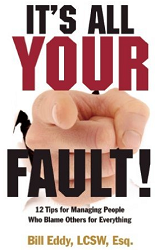
\includegraphics[width=\figwidth]{pics/17/6.png}
	\end{center}
\end{wrapfigure}
Seriously, EVERYTHING was our fault.

It was our fault that several members of Sciscitat's team had died during the battle in the evidence warehouse.

It was our fault that the traitorous Inquisitor had died before he could be questioned.

It was our fault that several extremely rare and valuable xenobiological specimens had escaped, died, or been turned into squigs.

It was even our fault that a several lightyear wide shadow had fallen across the warp, disrupting Astropathic communication, causing sub-sector wide political turmoil, and prompting the redeployment of several Imperial fleets to protect against a supposed hive-fleet incursion. 
(Okay, in retrospect putting the Daemonthrope in an Astropathic Sanctum might not have been the best idea, but how the hell were we supposed to know that? 
The closest things we had to experts on psi were Fio and Fumbles.)

Oh, and finally, it had apparently been our "inexcusably reckless" actions which finally gave Oak's enemies the ammunition they needed to bring charges of treason against him. 
So the whole entire current mess: 
the arrest orders issued for all of Oak's teams, the attacks on his allies under the cover of official investigations, the seizure of the research facility and Sciscitat's own imprisonment, and even Oak being forced to take his battleship into hiding; 
it was all OUR fault.

Or at least that's what Inquisitor Sciscitat and his minions thought. 
Personally, we blamed a combination of bad luck, everyone else being stupid, Orks, and the perverse nature of universe itself for at least eighty percent of all that. 
As for the others, the Magos didn't seem to care about anything other than his specimens, and for all his complaining, he actually seemed very interested in the Daemonthrope. 
And the Diplomacy adept, who'd inexplicably wound up in charge of the discussion, claimed it didn't matter either way, and encouraged everyone to focus on the next stage of their respective missions.

\begin{wrapfigure}{O}{\figwidth}
	\begin{center}
		
\includegraphics[width=\figwidth]{pics/17/7.png}
	\end{center}
\end{wrapfigure}
Our role in these "missions" was that of hapless go-fers. 


See, before the arrival of the traitorous Inquisitor and the Daemonthrope's astropathic jamming aura, Oak had sent orders which assigned us to Sciscitat's retinue for the duration of some vaguely-defined investigation. 
Since the Inquisitor thought of us as "a bunch of juvenile, tactless, indiscreet, and dangerously incompetent meatheads", and we considered him to be a socially inept cogitator weeny with delusions of genius, why we'd been paired up like this was a bit of a mystery, but the orders seemed genuine.

It belatedly occurred to us that our decision, back on our second-ever Inquisitorial assignment, to ever-so-slightly falsify then-Interrogator Scitatat's after-action report might have been a bad idea. 
Sure, before we'd edited it, the report had been full of accusations of incompetence and obstruction, and it had ended with a recommendation that we all be re-assigned to a penal legion… But maybe that was how all his reports were written, and the way we'd removed all mention of our antics and put our own performance down as "Nearly Adequate" had wound up looking like high praise in comparison. 
Or maybe, as Twitch now insisted, Oak had seen through the forgery on day one, and this was his punishment.

Anyway, whatever the reason we'd been assigned to the asshole, we had no choice but to stick to our orders. 
Well actually we could've told Sciscitat and Oak to stuff it and then went off to do our own thing, but there's nothing like knowing that the Inquisition has issued a warrant for your arrest to motivate a cooperative attitude.

So yeah, Inquisitor Sciscitat was our new boss, and his first orders were to "Stay out of my way, and Assist Magos Smith in any way possible." Which is why we spent the next few days fetching, carrying, and occasionally squig-wrangling for a tech-priest who, in a totally unexpected twist of fate, turned out to be completely nuts.

\begin{wrapfigure}{O}{\figwidth}
	\begin{center}
		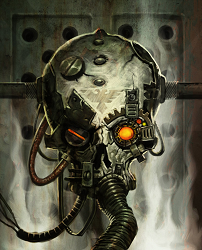
\includegraphics[width=\figwidth]{pics/17/8.png}
	\end{center}
\end{wrapfigure}
Well, maybe not COMPLETELY nuts, but that was only because the Magos was so far around the bend that he was re-approaching sanity from the opposite direction. 


First of all, it turned out that he wasn't actually the tech-priest that we'd seen walking around with the Inquisitor and Diplomacy Adept. 
It took a while, but after the third incredibly awkward conversation with the inexplicably unresponsive tech-priest, we finally figured out that it was actually the oversized servo-skull that was calling the shots. 
The tech-priest-looking body, as well as that giant man-beast we'd seen in the warehouse battle and a fair number of other freakish looking things, were something like a cross between a servitor and a full-body augmetic. 
He called them "Meat Puppets", which should tell you everything you need to know about the state of his mind.

At first some of us (mostly Tink) were rather curious about how a tech-priest winds up as a disembodied brain flying around controlling a horde of servitors and flesh-sculpted monstrosities. 
When Tink tried to press the Magos on the why and how of his servo-skulliness though, all he got was a vague comment about having done it to himself for political reasons and an assurance that: 
"Getting the brain out was the easy part. 
The hard part was getting the brain out." Then the Magos flew off cackling, only to return a few minutes later to scream at us (for about the fifteenth time) for killing his prize Eldar test-subject. 
Or maybe he'd been angry about the death of the lizard thing, or the group Bendies we let escape, or how his entire collection of genestealer cultists had been squigged. 
It all sort of ran together after a while.

\begin{wrapfigure}{O}{\figwidth}
	\begin{center}
		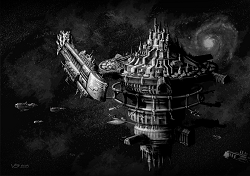
\includegraphics[width=\figwidth]{pics/17/9.png}
	\end{center}
\end{wrapfigure}
Putting the Magos' weirdness aside, the reason we were helping the crazy cogboy was that the brainy people had decided that the planet was no longer secure. 
The whole debatably-heretical research facility needed to be packed up and moved via the first available Imperial vessel. 
Which is to say, the Occurrence Border.

You can just imagine how thrilled the Captain and Ol' Bill were to find out their ship would be playing host to a xenobiological research lab, completed with an insane Magos Biologis, numerous psychically-gifted specimens, and the damned Daemonthrope they'd only just finally gotten rid of. 
The only reason they limited their complaints to bitter grumbling (as opposed to orbital strikes), was the Occurrence Border's supply situation and the awkward tactical problem which had resulted from it.

See, after such a long and hard journey without resupply, the Occurrence Border was out of just about everything. 
So when it finally used the last of its fuel (and the recoil from its macro-turret) to slow down enough to dock with the small refuelling station orbiting above the facility, its Captain was in a rather ruthless state of mind. 
The ex-naval officer, having had it up to here with politely asking, begging, and (Emperor forbid) paying for supplies that were rightfully his to requisition, had broadcast his ship's Inquisitorial credentials and announced his intention to commandeer EVERYTHING. 
Not everything as in "everything you can spare", literally everything. 
As in down to the crew, atmosphere, and the station itself.

The locals objected to this of course, complaining loudly that this sort of looting wasn't even remotely within the legal limits of the Captain's Inquisitorial charter, and called for aid from the only other ship in the system: 
the light cruiser which had brought the recently-squished Inquisitor and his arrest team.

\begin{wrapfigure}{O}{\figwidth}
	\begin{center}
		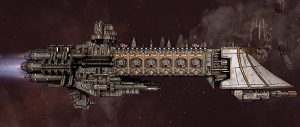
\includegraphics[width=\figwidth]{pics/17/10.png}
	\end{center}
\end{wrapfigure}
The light-cruiser was a standard naval vessel that had been commandeered by the traitorous Inquisitor to provide transport and overwhelming fire support for his arrest team. 
After the initial excitement of its arrival the ship had just sat in orbit, serving as protection, Astropathic communication provider, and storage for items that were too large to fit in the evidence warehouse; 
such as the facility's shuttles and a small cogitator-filled normal-space vessel that had been in orbit when they'd arrived. 


It'd been a nice boring assignment for them right up until their Astropaths lost contact with the rest of galaxy. 
Then, while they'd been off at the edge of the system, futilely attempting to outrange the Astropathic jamming we'd unknowingly been broadcasting ahead of us, the Occurrence Border had arrived. 
By the time they managed to get back to the facility their Inquisitor was very dead. 
Left to their own devices, they probably would have just destroyed the Occurrence Border and blockaded the research facility until the arrival of further orders. 
Fortunately for us though, the Deathwatch Apothecary had claimed command as the technically-ranking survivor of the dead Inquisitor's retinue, and told the ship to stand down. 


The light-cruiser had sat in orbit, waiting for the Apothecary to finish his business on the planet, until the Occurrence Border started its looting spree and the Station requested their aid. 
The ship's captain, being mindful of all the Inquisitorial bullshit going on, voxed the Apothecary for orders, and the Space Marine kicked the problem over to Sciscitat, who probably made some sort of smug "just as planned" comment before voxing the Occurrence Border. 
The Captain was basically asked whether he'd prefer to transport on the Magos and his lab, or go toe-to-toe with a ship ten times more combat-capable than his own. 
The Captain went with the former, but it was a close thing.


\begin{wrapfigure}{O}{\figwidth}
	\begin{center}
		
\includegraphics[width=\figwidth]{pics/17/11.png}
	\end{center}
\end{wrapfigure}
So, while shuttle after shuttle carried xenobiological specimens, techno-heretical research equipment, and bizarre servitors into orbit, the Occurrence Border's entire crew flooded into the little station, and under the guidance of Ol' Bill and his engineers, set about looting the place more thoroughly than even the most determined Freeboota could manage. 
Every scrap of fuel, supplies, and equipment aboard the station was commandeered. 
The entire crew, down to the dependents, servitors, and family pets, was rounded up by the press-gangs and given a once-in-a-lifetime chance to earn their passage out of the system as an indentured voidsman. 
Finally, the handful of backwater tech-priests and Administratum scribes that ran the place (and who were technically exempt from naval conscription) were given a choice between "voluntarily" joining the crew or staying behind as Ol' Bill and his engineers sucked out the atmosphere, cut the station into manageable chunks with lance-fire, and then strapped the pieces to the Occurrence Border's hull like hunting trophies. 


Of course we weren't personally around to see the entirety of the looting spree: 
we actually only stayed in the system for a few days before our new boss decided it was time to go, and during that time we were all very busy helping the Magos move his lab. 
Well, I say "we", but honestly, certain members of the team didn't pull their weight during the whole packing process.

For instance, Aimy dodged her fair share of the work by collapsing in a heap about ten seconds after the Astartes-grade painkillers she'd been given for her MASSIVE scalp wound wore off. 
She wound up spending the rest of her time in the facility lying around alternately moaning and swearing at the rest of us, and rode up on the first shuttle back to the Occurrence Border.

\begin{wrapfigure}{O}{\figwidth}
	\begin{center}
		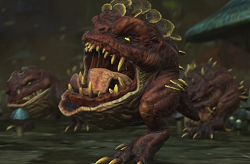
\includegraphics[width=\figwidth]{pics/17/12.png}
	\end{center}
\end{wrapfigure}
Doc, no doubt encouraged by Aimy's bad example, announced that he was too busy with medical things to do an honest day's work. 
At first he insisted that keeping Aimy's head from getting infected and falling off took priority over carrying boxes and herding squigged genestealer cultists. 
Then he just had to help the Apothecary reattach his arm and get Heart and Grumpy Marine into stasis. 
And after that it was all "I've got to transfer my information on Sergeant Gravis' condition, and fix the scalpel wound in my face", the lazy bastard.

Sarge wasn't any help either: 
he kept running off to chat with the Diplomacy and Cogitator Adepts about "conspiracies" and "politics" and "how did you know the Xenology Adept was a traitor before you shot him". 
This newfound laziness was a perfect example of what promotion over the rank of sergeant does to a guardsman.

The worst of all were Tink and Jim: 
they were so desperate to avoid some honest work that they actually left the whole planet, taking our shuttle back up to the Occurrence Border before the ship had even finished decelerating. 
Jim claimed he had to go warn Hannah and the tech-acolytes that someone called "The Fleshsmith" was still alive and would be coming aboard, so he might've had an actual reason, but the only excuse Tink had was that he needed to go hide Fio before the annoying little xenos wound up in the Magos' specimen collection. 
Of course that turned out to be a load of bullshit. 
Firstly, the Magos found his super-secret hiding place all of ten minutes after arriving on the ship. 
Secondly, all the Magos did upon seeing the annoying little xenos was point out that Tau were genetically uninteresting, and ask whether the room was the xenotech garbage dump. 
He then tossed the battered remains of Spot (sans-wraithbone, he was apparently keeping that for himself) onto the floor and left without waiting for an answer. 
So yeah, time well spent.

\begin{wrapfigure}{O}{\figwidth}
	\begin{center}
		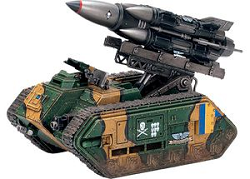
\includegraphics[width=\figwidth]{pics/17/13.png}
	\end{center}
\end{wrapfigure}
The point is that, despite it being our Inquisitorialy-assigned task, the only members of the team that actually did any real Magos-moving were Nubby, Twitch, and Fumbles. 
While everyone else made up excuses, the three of them slaved away, carrying boxes and recapturing escaped specimens while being screamed at by a crazy cogboy's disembodied head. 
They even used their own personal free time to collect desperately needed supplies for the team, and did they get thanked for their efforts? 
No! 
It was all: 

\greentext{>"We're not going to PAY you for returning our pulse weapons." }

\greentext{>"Deathwatch-issue hand weapons and wargear cannot be claimed as legitimate battlefield salvage."}

\greentext{>"That bolter wasn't 'gifted' to us. 'Gifting' is not, and never has been, an ancient Space Marine tradition. If you know where it landed, go get it and give it back to the Apothecary."}

and
\greentext{>"It doesn't matter if they're not going to need them anymore, we're not taking any of the facility's anti-orbital missiles with us. Even if, no, ESPECIALLY if Twitch says he can convert them to be man-portable."}


Anyway, putting aside matters of laziness and ingratitude, after a few days almost everything was packed up and word came down Sciscitat had finished digging through the dead Inquisitor's underwear drawer, or whatever he'd been doing, and it was time to get ready for our mission. 
Not that we knew what the mission even was: 
the closest thing to a briefing we'd gotten was our initial meeting with the Inquisitor after we pulled him out of stasis and collected those of his retinue who'd survived the evidence-room battle.

\begin{wrapfigure}{O}{\figwidth}
	\begin{center}
		
\includegraphics[width=\figwidth]{pics/17/14.png}
	\end{center}
\end{wrapfigure}
That meeting had been singularly unpleasant. 
Aside from all the aforementioned yelling, realizing Sciscitat was our new boss had come as a nasty shock; 
he'd been an Interrogator last we'd seen him, back when he'd led our second ever Inquisitorial mission. 
Back then he'd been a self-important data-analysis weenie, who sat around on a small normal-space corvette stuffed to the bulkheads with cogitators, while his team did the dirty work of gathering intel and executing the over-complex plan he cooked up. 
Picture the most arrogant, annoying intellectual you've ever met, then add a fondness for self-praise filled meetings and berating his minions, and finally top it off with just enough analytical genius for him to get away with all this. 
On our previous mission he'd done a decent enough job of unraveling the mystery we'd been sent to solve, but in our opinion he was a terrible Interrogator, and never should've been allowed to lead field ops.

Of course that had been a while ago, and time changes everyone. 
He wasn't an arrogant little shit of an Interrogator anymore. 
Now he was an arrogant moderately-overweight shit of an Inquisitor. 
Oh, and this time he was convinced that we were dangerously incompetent from the outset.

Along with his charming self, the Inquisitor had also brought some of our former teammates along. 
The psychic eavesdropper, Snitch, was just as weasel-like and eager to report our thoughts to his boss as we'd remembered, though he'd acquired a nasty skin affliction somewhere along the line, possibly due to way he constantly used his psychic powers. 
The other psyker to survive that mission, Face, seemed little buffer than we remembered and carried a force-sword now, and he'd added a prissy little mustache to his pretty-boy look. 
Finally, noble-born social infiltrator chick was just as posh and assassin-y as we'd remembered, but had also acquired a bunch of Cyber-Mastiffs and been promoted to Interrogator.

\begin{wrapfigure}{O}{\figwidth}
	\begin{center}
		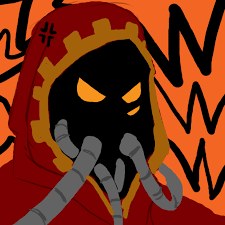
\includegraphics[width=\figwidth]{pics/17/15.png}
	\end{center}
\end{wrapfigure}
On top of the familiar faces, the Inquisitor's retinue included several combat specialists. 
Well, at least it had before the whole evidence-room battle, now it was down to just a Cleric with a brand-new augmetic arm and a Sororitas-style bolter instead of the usual flamer, and a wiry guy with far too many knives who literally had "Deathcult Assassin" tattooed on his forehead. 
The final member of the team was the Tech-Priest who maintained the Inquisitor's surveillance toys; 
his chief distinguishing feature was that he hated us.

Actually, hating us was pretty universal. 
Snitch, Face, and the Interrogator all shared the Inquisitor's theory that were completely unfit for Inquisitorial service, and the Assassin and Cleric bore a serious grudge over how those of us in the evidence room had just edged around the big battle instead of chipping in. 
We tried to explain about how important dealing with the Daemonthrope had been, and how we totally would've helped them if we'd known we'd have to actually work with them later, but they didn't seem interested in listening. 
Their hatred was more of a mix of disgust and resentment though; 
the Tech-Priest's was the real deal. 
See, he was one of those hardcore religious types, and our collection of xenotech weapons (especially Tink's Tau-hybrid plasma gun) did NOT go over well with him. 
He fervently believed that we should all be killed in horrifically violent ways for our blasphemy, and while he wasn't quite crazy enough to act on that belief, he did make sure to regularly remind us that we were all damned to robot-hell.

So yeah, these people who respectively thought we were dangerously incompetent, blamed us for the death of their comrades, and wanted to burn us at the stake (or whatever the cogboy equivalent is), were the guys we were supposed to "accompany and assist on their mission". 
Thanks Oak.

\begin{wrapfigure}{O}{\figwidth}
	\begin{center}
		
\includegraphics[width=\figwidth]{pics/17/16.png}
	\end{center}
\end{wrapfigure}
As far as what that mission was, all the Inquisitor was willing to tell us was that he had been sent to investigate an Imperial world that was believed to be a stronghold of The Conspiracy. 
This wasn't exactly a wealth of information, but it was enough to convince us that we wanted absolutely NOTHING to do with it. 


Seriously, he was proposing going to a world that was under control of what had been described to us as cabal of traitorous Inquisitors, you know, those guys who can requisition everything up to and including an EXTERMINATUS? 
I mean, as nasty as Inquisitors (especially ones mucking around with daemonic powers) can be on their own, it's their massive, nearly-unquestionable authority that really makes them really scary. 
Having that on your side is great, not only not having it, but actually going up against it? 
Not so much. 
What Sciscitat was proposing wasn't a stealth mission, it was a "if someone even suspects you an entire planet will hunt you down" mission, and that was just the BACKDROP. 
Emperor knew what sort of crazy shit the actual investigation was supposed to be centered around… oh and let's not forget that our teammates, the only people on the whole planet we could trust to watch our backs, actively hated us.

Okay, maybe that's overselling things a bit, but it really was an unpleasant sounding mission, and we responded to it in the traditional guardsmanly fashion, which is to say that we desperately attempted to weasel our way out of our orders. 
Sadly, the entire situation turned out to be remarkably weasel-proof. 
Oak's orders attaching us to Sciscitat they were far too simple and direct for us to get away with creatively misinterpreting them, and we didn't have any better luck trying to get Sciscitat to dismiss us: 
as distasteful as the man found working with us, he seemed to consider a "suggestion" from Oak roughly on par with a divine mandate. 


\begin{wrapfigure}{O}{\figwidth}
	\begin{center}
		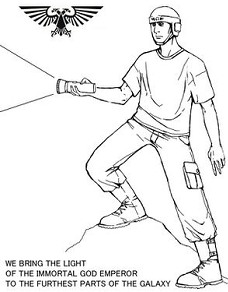
\includegraphics[width=\figwidth]{pics/17/17 Large.png}
	\end{center}
\end{wrapfigure}
Of course divine mandates tend to be open to a bit of interpretation; 
while Sciscitat was dead set on bringing us along, he made it clear that he wouldn't trust us to organize a piss-up in a brewery, much less perform an Inquisitorial investigation. 
This had led to our official designation as dumb muscle, which was just fine with us, but it had also led to The Rules, which were less so. 
Sciscitat had described them to Sarge's face as an attempt to "idiot proof" our part of the mission, and almost gleefully put the tech-priest in charge of writing them. 
That of course led to a lot of arguing, Tink's little aborted attempt at mutiny, and a desperate scramble to find where all of our old weapons had gotten to, which ended in even more yelling.

All of us had known that our supply of non-rechargeable munitions had been running low for ages: 
the grenades and detpacks had lasted almost to the end thanks to Twitch's hoarding, but the existence of things like krak-missile launchers was just a vague memory, and Sarge's ammo-less grenade launcher had been traded away to some tech-acolyte building a combat servitor long ago. 
What had been less well-known, was that the hotshot lasguns which had been shelved in favor of our pulse-weapons had been marked as "extra-knee-us" and left in the possession of a certain Ratling black marketeer in favor of more lucrative items. 
Nubby's justifications about how he'd been planning to just buy us new ones if we ever needed them didn't go over well with any us. 
Long story short, we wound up armed for our upcoming Inquisitorial mission with nothing but our sidearms and standard-issue lasguns from the Occurrence Border's armory, which sat especially poorly with Tink, who hadn't used one since basic.

Anyway, word came down that the Inquisitor had finished his pre-mission whatever and it was time to move out, so we packed up our measly armament, and for the first time since we'd left Tau space, said goodbye to the Occurrence Border. 


\begin{wrapfigure}{O}{\figwidth}
	\begin{center}
		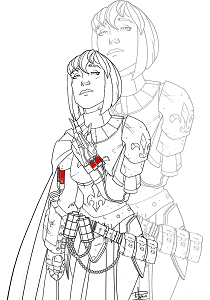
\includegraphics[width=\figwidth]{pics/17/18.png}
	\end{center}
\end{wrapfigure}
While we weren't going to miss the horrible pile of warp-tainted scrap we'd been riding around on, its crew was another matter, so on our way out we paid a few visits to say goodbye (and make sure all of Twitch's little "surprises" had been disarmed, or at least documented). 


The Captain and Ol' Bill were too busy to do more than tell us not to get killed, Jim promised to look after our stuff and make sure nobody dissected Fio, and Hannah thanked us for not trying to bring Jim. 
The Diplomacy Adept, who'd somehow wound up in charge of everything, asked Sarge to at least TRY to work with Sciscitat, and said he'd take care of our official report to Oak, since the Occurrence Border would be proceeding directly to the Inquisitor's hiding place. 
As for the other Adepts: 
the Cogitator Adept wasn't in his room and we didn't actually care enough to try and find him, and the Xenologist was still dead.

When we all visited the medbay Aimy wasn't really coherent enough to say goodbye. 
Unlike her previous two head injuries, this time every scrap of skin above her nose needed to be regrown, so her head was pretty much this giant pile of bandages and (this being a Sororitas-developed procedure after all) prayer seals. 
Aimy was too doped up on painkillers to really understand anything, but Sarge tried to fill her in on the situation. 
The rest of us just stood around speculated on whether the markswoman would still obsess over her hair, since this time her entire scalp would be regrown Sororitas-white, and whether there was some sort of energy-attack-attracting magnet embedded in her skull somewhere (Sister Valerie said she'd check). 
As for Doc's girlfriend, the two of them had already said their disgustingly sappy goodbyes, and all she had for the rest of us was a promise that returning without our medic would just be a very slow and painful method of suicide.

\begin{wrapfigure}{O}{\figwidth}
	\begin{center}
		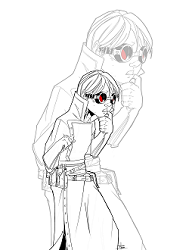
\includegraphics[width=\figwidth]{pics/17/19.png}
	\end{center}
\end{wrapfigure}
Our final stop was the poorly-hidden lab where Fio was setting all his gear back up with Fumbles' help. 
While Tink pulled Fio aside for a final go over of the plans for Spot's third rebuild (being used as a bludgeoning weapon by a Space Marine isn't as bad as a nuclear blast, but it's pretty close), the rest of us said goodbye to our favorite psyker. 
We'd really wanted to bring the little guy, but the Inquisitor had flatly refused, and we couldn't really argue. 
When you get down to it, a psyker who uncontrollably broadcasts his emotional state and has problems controlling his powers at even the best of times has no place on a stealth mission. 
Also, he didn't really get along with the Inquisitor's psykers, especially Snitch, who claimed that Fumbles was like a cross between a painfully-loud Vox unit and an unexploded artillery shell.

Anyway, it sucked leaving Fumbles behind, but at least he took the news better than we'd expected. 
There was some initial moping, but he actually seemed pretty relieved not to be going to a heavily populated Imperial world where he'd have to worry about religious fanatics lynching him for having oversized eyes or just being a psyker. 
Also, he said it would be nice to get a break from constant life-and-death struggles, or at least as close to one as you can get as a psyker on a warp-tainted scrapheap of a ship. 
We wished the little guy luck, Nubby tried to give him a list of not-quite-legal things to trade for if the ship made any stops, Sarge hit Nubby, and then we rounded up Tink and left the Occurrence Border. 


It should've been a happy moment: 
there were few things we'd wanted more than to leave that horrible deathtrap… But honestly, given a real choice between whatever shit-show of a mission was waiting for us and a five year stint on the Occurrence Border, we probably would've taken the latter. 
It just goes to show that the Inquisition can, and probably will, ruin anything.

\begin{wrapfigure}{O}{\figwidth}
	\begin{center}
		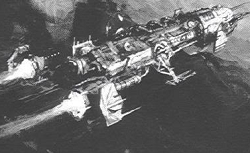
\includegraphics[width=\figwidth]{pics/17/20.png}
	\end{center}
\end{wrapfigure}
The shuttle that took us to the Inquisitor's ship was one of his. 
Officially this was because all of the Occurrence Border's were busy strip-scavenging the station (even Tink's repaired and de-fungused stealth shuttle was used, though everyone on it kept their void-suits on), but it probably had more to do with how much harder that made it for us to sneak anything aboard. 
It was unnecessary of course, we had given our solemn word to follow their stupid rules after all (and we knew from experience how hard it was to get stuff past Snitch), but that didn't stop that damned Tech-Priest from inspecting our gear and baggage before he let us onto the Inquisitor's ship

The Inquisitor's ship was the same one he'd had back during our previous mission: 
a little corvette that was mostly just there to carry his massive cogitator array. 
It was small, cramped, unarmed, and didn't have a warp-drive, all of which seemed like major design flaws to us, but for some reason we hadn't been consulted when they'd built the thing. 
Unlike a proper ship, it was crewed by only a couple dozen professional voidsmen and tech-priests, who generally treated us like a visiting friend's incontinent little yappy dog (We got the distinct impression that they were still unhappy about the time we'd propped a dead psyker up in one of the bathrooms).

Anyway, lacking a warp-drive, the Inquisitor's ship depended on larger vessels to carry it between systems. 
Unfortunately, the only such ship present (aside from the Occurrence Border, which wasn't going our way) was the light-cruiser which had brought the arrest team into the system. 
This led to the very awkward situation where we had to ask for a lift from the ship that had recently boarded and impounded our vessel. 
Well, that is to say it was awkward for the Inquisitor and his minions, we dismissed the whole situation as "Not our problem" and set about making ourselves as comfortable as possible in the cramped quarters we'd been assigned.

\begin{wrapfigure}{O}{\figwidth}
	\begin{center}
		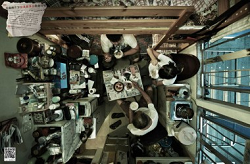
\includegraphics[width=\figwidth]{pics/17/21.png}
	\end{center}
\end{wrapfigure}
Our time aboard the Inquisitor's ship was pretty unpleasant. 
The problem wasn't that he and his crew did anything to antagonize us, they just ignored us in the sort of put-upon way usually reserved for racist old relatives visiting for the holidays, and we did likewise. 
So really, it was just like all of our missions before Sarge's forced promotion, except for one big difference: 
nobody let us do ANYTHING.

We'd gotten used to being on a ship that suffered near-continuous warp-phenomena, equipment failures, xenobiological infestations, and minor daemonic incursions during even the smoothest of transits. 
There'd always been something that needed shooting, fixing, or fortifying, or a mission to plan for, or some sort of Nubby-related scam going on. 
Compared to that, travelling on the Inquisitor's ship was just, well, boring. 
Not that we were against being bored mind you. 
Life in the Guard is pretty much long periods of boredom punctuated by moments of sheer terror and Orks. 
So we were used to boredom, in fact we loved it, because the alternative tended to involve xenos, heretics, superior officers, or some combination of the three trying to kills us. 
It was just that we didn't have enough space to enjoy our boredom.

See, since the Inquisitor thought we were borderline-retarded and therefore a massive hazard to operational security, we weren't invited to his stupid meetings. 
This was fine by us: 
we'd hated the meetings, and were perfectly okay with him just handing us a briefing when we got to wherever we were going. 
Unfortunately in addition to not-inviting us, Sciscitat ordered us to stay in our quarters during all hours in which a meeting might be held, presumably in case we overheard something and somehow managed to blab it to the enemy despite being in the middle of bloody warp space.

Said quarters consisted of a single shared bunk-room and the Inquisitor's "working hours" lasted from 0700 to 2300. 
It was a miracle that nobody was killed.

\begin{wrapfigure}{O}{\figwidth}
	\begin{center}
		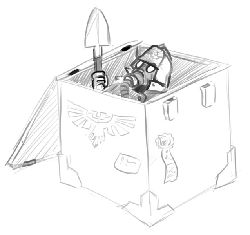
\includegraphics[width=\figwidth]{pics/17/22.png}
	\end{center}
\end{wrapfigure}
Let me tell you, twenty square meters with low ceilings is NOT enough space for five guardsmen. 
Well technically, according to the Astra Militarum regulations book which the Inquisitor gleefully cited when we complained, it's enough space for either eight standard-issue Guardsmen, twelve Ratling auxiliaries, four Ogryn, or twenty-six and a half Kriegers, but those regs are "ideal circumstances" Munitorum bullshit and everyone knows it. 
Except the Krieger part.

Anyway, sixteen hours a day confined in a small room with Nubby, a chronic whiner relearning basic las-gun use, a hyperactive paranoid with no perimeter to secure, Nubby, a man who just would not shut up about his absent girlfriend, the grumpiest noncom in several cubic lightyears, and Nubby was just too much. 
The one small mercy was that Aimy and Fumbles weren't along, otherwise we might not have even made it through the first day. 
As it was we were all just about ready to strangle each other by the end of the third.

Of course we didn't just sit around waiting for things to reach that point, it was obvious from the get-go that we weren't going to survive the trip unless we got a little more space. 
Sarge wasted a fair bit of time trying to talk Sciscitat around, but when that failed we decided to just quietly annex a few rooms which we felt were… underutilized. 
Unfortunately, some of ship's crew noticed us hauling our stuff into the rooms of the guys who'd gotten themselves killed during that shit-show at the research facility (C'mon, it's not like they needed all that space anymore). 
When the Inquisitor and all his minions showed up to yell at us Sarge made some very good points about about efficiency and the importance of keeping morale up, but since Nubby and Tink were rooting through the deceased's stuff behind him, his arguments didn't go over very well.

\begin{wrapfigure}{O}{\figwidth}
	\begin{center}
		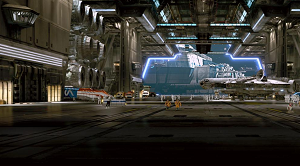
\includegraphics[width=\figwidth]{pics/17/23.png}
	\end{center}
\end{wrapfigure}
Our second attempt to expand our quarters was a bit more direct, and consisted of Tink rigging up a lascutter and cutting through the wall between us and a the storage room next-door. 
Sadly, he only got a quarter of the cut done before that damned tech-priest burst in and started screaming at us, and the rest of the retinue showed up before we'd decided whether we could get away with shooting the cogboy and blaming it on our combat reflexes. 


That little incident ended with yet another painfully long lecture from the Inquisitor, which was capped off with a promise to kick us off his ship if we disobeyed orders again. 
Sarge, who was reaching critical levels of grumpiness at that point, began to respond with something along the lines of "You can try", but reconsidered as the exact nature of that threat dawned on him, and wound up struggling to maintain a poker face (and mind) while the Inquisitor ranted. 
When the lecture finally ended with Sciscitat and his minions storming out to return to their meeting, Sarge asked the rest of us how we felt about taking the Inquisitor up on his "offer".

That night a note was taped across from the Inquisitor's door, regretfully informing him that we'd violated his orders against screwing with the ship's systems by disabling the forward airlock's alarms, and since he was asleep at the time, we'd undertaken to kick ourselves off the ship for him. 
Then we'd gathered our gear, donned our voidsuits, and one short walk through a depressurized assault-shuttle bay later, we were arguing with a bunch of confused navy armsmen about whether we honored Inquisitorial guests or a hostile boarding party.

\begin{wrapfigure}{O}{\figwidth}
	\begin{center}
		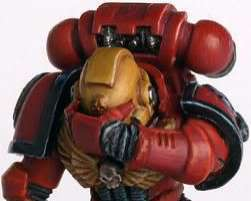
\includegraphics[width=\figwidth]{pics/17/24.png}
	\end{center}
\end{wrapfigure}
After everyone stopped pointing weapons at eachother (except for Twitch), it only took us showing off Sarge's Interrogator rosette to convince the armsmen to kick the problem upstairs. 
Talking our way through the succession of Navy officers wasn't too hard (even if they are unquestionably inferior to the Guard, the Navy does at least speak the same language), and before long we were escorted to the section of ship that had been claimed by the Deathwatch Marines.

The Apothecary, who'd traded his damaged Power Armor for blue and gold comet-embroidered medicae robes, greeted us at the door. 
The Marine obviously wasn't overjoyed to find us on his doorstep asking if we could crash on the equivalent of his couch for a few weeks, but we'd apparently earned some respect from him and his team during the battle, because he let us in with no more than a pained sigh and a comment about how "Monitoring for stowaways does not fall under the purview of the Deathwatch". 
The Apothecary directed us towards the quarters which had belonged to the squished Inquisitor and his retinue, told us not to bother him or his patients, and that was it. 
No request for an explanation, or rules about what we could or couldn't do, just that special brand of apathy that is the hallmark of a good barracks-mate. 
If he'd been a Guardsman we'd have bought him a crate a beer, but since he was a monastic super-soldier older than all of us put together, we settled for staying out of his way.

\begin{wrapfigure}{O}{\figwidth}
	\begin{center}
		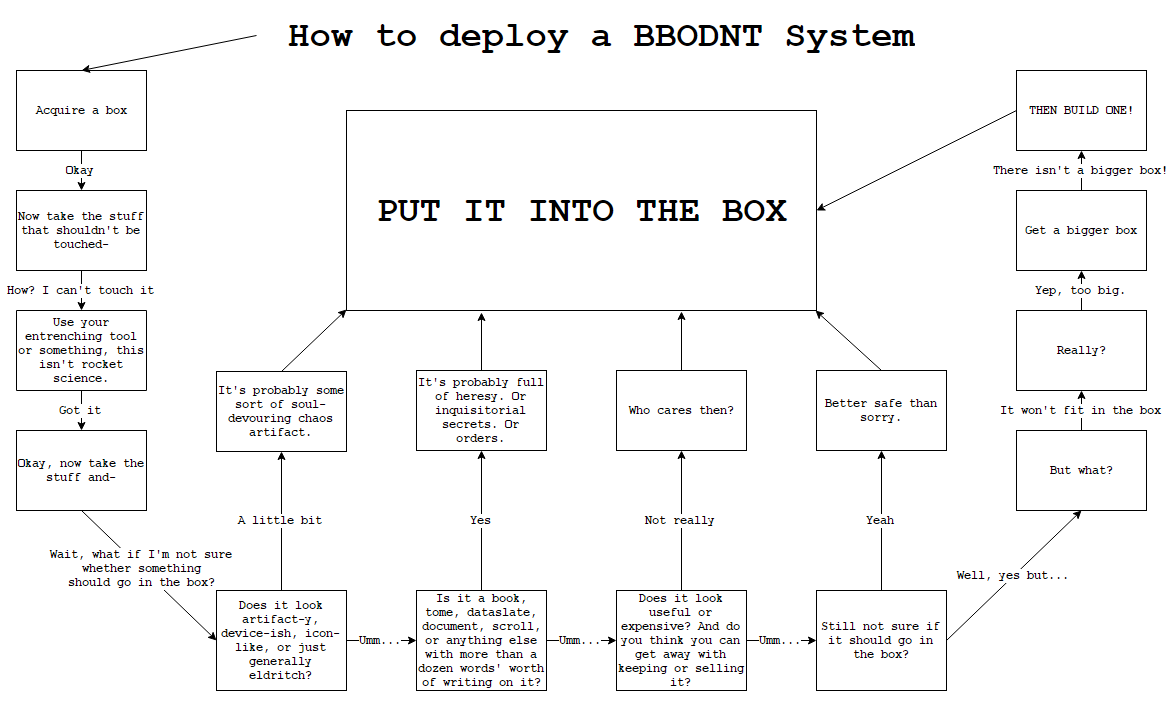
\includegraphics[width=\figwidth]{pics/17/25-large.png}
	\end{center}
\end{wrapfigure}
We made ourselves comfortable in short order. 
Twitch found a comm system and put in a requisition for a staggering amount of explosives, rations, and other supplies from the light-cruiser's stores. 
Nobody else had expected this to work, but since the ship's quartermaster was under the impression that the order was on behalf of the big scary Space Marines, the stuff was actually delivered. 
Seeing this, Nubby put in his own requisition for "all da money you got", which was met with a bit more skepticism. 
Sarge barely managed to bluff the Quartermaster off without the Apothecary finding out, and announced that the next person to even talk to someone from the light-cruiser's crew would be sent back to Sciscitat's ship.

Fully resupplied for the first time in ages, Twitch made a horrible, but very secure, mess of our new quarters. 
As a side note, most of this stuff was left in place when we reached our destination on account of the Inquisitor's silly twenty-kilo limit, and because nobody felt like cleaning it up. 
An official complaint  from the ship's captain caught up with us a few months later, just in time to be used as evidence in fact, but it was really only a minor sidenote compared to the rest.

While Twitch fortified, Nubby and Tink gave our new quarters a thorough looting. 
Now, the previous occupants having been an Inquisitorial team (and possibly a traitorous one at that), there was a fair bit of stuff that could be loosely described as "eldritch". 
Your average Inquisitorial team would've gotten excited and started sifting through the stuff search of intel or whatever, but honestly, when was the last time you heard of digging through a pile of eldritch shit working out well for someone? 
So per rule \#38 of Greg Sargent's Guide to Not Dying in Inquisition, we employed The Big Box of Do Not Touch. 
(If you're unfamiliar with this technique, basically what you do is you take a big box, put all the weird stuff into it, and then Do Not Touch it. 
Very complex.)

\begin{wrapfigure}{O}{\figwidth}
	\begin{center}
		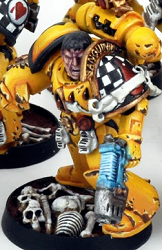
\includegraphics[width=\figwidth]{pics/17/26.png}
	\end{center}
\end{wrapfigure}
Most of the stuff that wasn't Boxed found its ways into Nubby's grubby pockets, the only notable exception being an oversized plasma pistol that went to Tink, which the two of them claimed had belonged to the arrest-team's Ogryn. 
Upon seeing the weapon and hearing the explanation, Sarge weighed our need for a heavy-ish weapon (not to mention how annoying it had been trying to re-teach Tink basic lasgun use) against how angry certain people could get. 
In the end he decided not to ask any questions he didn't want answers to. 
Such as why nobody else had seen this Ogryn during or after the warehouse battle, or why anyone would ever give an Ogryn such a notoriously finicky weapon, or why: 
"PROPERTY OF THE LAMENTERS SPACE MARINE CHAPTER" was stamped along the pistol's side.

After the "cleaning" and fortifying we settled into a nice comfortable routine that mostly consisted of naps, PT, gear maintenance, a few personal projects, and more naps. 
Twitch and Nubby did their best to keep out of trouble and carefully planned out what supplies would be brought with us when we eventually arrived. 
Tink spent most of his spare time reconfiguring his oversized plasma pistol into something that could be used by someone with normal-sized hands and putting together replacements for all his Tau-tech toys. 
Sarge, along with being generally sergeanty, waited a few days for tempers to cool then started making regular visits to Sciscitat's ship to see how things were going. 
Most of the visits consisted of him just being told that there still wasn't anything he needed to know and to go away, but he was occasionally given little tidbits of nearly-useless information. 
Such as the fact that our destination was some shit-hole of a Hive World, that Oak still hadn't been caught, and someone or other had finally noticed the squished Inquisitor was missing. 
Sarge reciprocated by dumping the Big Box of Do Not Touch in Sciscitat's airlock. 
He was not thanked for this.

\begin{wrapfigure}{O}{\figwidth}
	\begin{center}
		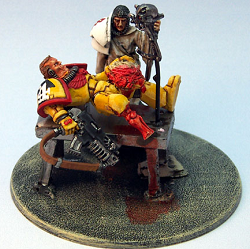
\includegraphics[width=\figwidth]{pics/17/27.png}
	\end{center}
\end{wrapfigure}
The odd man out in all this was Doc. 
Instead of relaxing while he had the chance like a proper guardsman, the medic went and practically begged the Apothecary to let him assist in the treatment of Sergeant Gravis and the wounded Deathwatch Marines. 
Doc must've earned some actual respect from the Astartes for keeping Gravis alive, or maybe his display of fanboy-ism was just too much to ignore, because the Apothecary eventually accepted and our medic was temporarily promoted to Volunteer Nurse and Janitor. 
He was also made to swear this oath not never talk about any of fancy-pants medical procedures he assisted in (which the we were thankful for, since it spared the rest of us a whole lot of disgusting medical stories), but he was allowed to update us on the status of the three Space Marine patients.

According to Doc, Heart and Grumpy were out of stasis and being kept in an induced coma. 
Between them they were going to need four augmetics, a dozen replacement organs, over a hundred hours of bone-realignment surgery, and a few months of bed-rest, but were expected to make a more or less full recovery. 
Sergeant Gravis was obviously in worse shape, but had at least been cleared of the Tyranid biotoxin by some Space Marine techno-magic, and had finally been removed from his damaged Power Armor. 
Doc said the Apothecary wasn't quite sure if he'd be returning to duty (mentioning something about Gravis' chapter being undersupplied), but had started installing neural links for some type of specialized full-body augmetic anyway. 
We figured that sounded like as good an ending for him as was possible, though we were all a little unclear on what sort of augmetic a "Sarcophagus" was.

Anyway, asking about the Space Marines was the closest thing to work most of us did on the trip, so we were all in a pretty good mood when the light-cruiser finally reached our destination and we made our way back to Sciscitat's ship.

\begin{wrapfigure}{O}{\figwidth}
	\begin{center}
		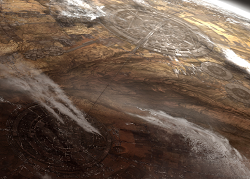
\includegraphics[width=\figwidth]{pics/17/28.png}
	\end{center}
\end{wrapfigure}
Thankfully, it only took a single day of cramped normal-space travel to reach orbit over our destination, the hive-world Haarlock's Wager. 
Or, to use its full name, Joseph Haarlock Sucks At Cards. 
We were advised not to discuss the planet's name, or the names of its primary hives, with the locals. 
It was apparently a touchy subject. 


Upon reaching orbit we were subjected to that most wonderful of experiences: 
a customs inspection. 
Which explained all that stuff about what we could or couldn't bring, even if didn't explain why the Inquisitor hadn't just told us the reason beforehand. 
Maybe he didn't want us trying to solve the problem ourselves.

Anyway, on a normal mission the Inquisitor would've flashed his rosette and that would've been that, but Sciscitat apparently felt that wasn't discreet enough. 
By the time we'd hit orbit, he and his minions had done some sort of cogitator stuff to convince the locals that our ship belonged to a local asteroid-mining syndicate, and even dug out some business suits and scribe robes for everyone but us to wear. 
We were just given little insignias to put on our armor and asked not to accidentally kill any inspectors. 
Between all that and some gentle psychic manipulation from Face and Snitch, the inspection went off without any significant hitches. 
Though there were an awkward few minutes when they insisted on going through the pile of stuff Nubby had brought back from the light-cruiser. 
Luckily there weren't any laws against having a bunch of second-hand small valuables and expensive clothing (mostly of the feminine variety), and while there probably was one against ripping an all-in-one kitchen and laundry unit out of one's quarters on an Imperial Navy Vessel, transporting it was entirely legal.

Once the inspectors were packed away there was another day of cogitator stuff and meetings, and then we were handed our orders, packed aboard a shuttle, and sent down to do some Inquisiting.

\begin{wrapfigure}{O}{\figwidth}
	\begin{center}
		
\includegraphics[width=\figwidth]{pics/17/29.png}
	\end{center}
\end{wrapfigure}
Well, actually it wasn't so much "Inquisiting" as "sitting around in a van". 
See, The Inquisitor's investigative techniques hadn't changed since his promotion. 
He still sat around on his ship with his precious cogitators, pouring through data gathered by his psykers, spy toys, and socialite minions until some clue or other caught his attention and he sent out his sneakier henchmen. 
Our role in this was that of emergency armed backup; 
"emergency" in this case meaning that they'd tried literally everything else short of an exterminatus. 


Every morning four vehicles would exit the mid-level hab-block which served as our home base The first was the scan-van, holding Snitch, the Tech-Priest, and all their spy toys, and typically piloted by the Cleric. 
Then there was a pair of sporty little anti-grav vehicles which Face and the Interrogator used to get to whatever up-hive social event they were nosing around that day. 
The final vehicle was an acid-stained junker of a van bearing the logo of a Soylens Viridians collection service, which had apparently been sold after its cooling system failed while hauling a full load, and was occupied by five extremely grumpy guardsmen.

These elevated grumpiness levels had more to do with our assignment than the deliberate shittines of our vehicle. 
It wasn't that we particularly minded being relegated to backup, and we were only moderately unhappy about the fact that we were STILL hadn't been told what the actual mission was (after all, it wasn't like we wanted to go out there and do all the cloak and dagger nonsense ourselves). 
No, the thing that had our collective panties in a twist was that we were expected to spend about twelve hours a day DRIVING A GROUND VEHICLE around a HIVE CITY.

\begin{wrapfigure}{O}{\figwidth}
	\begin{center}
		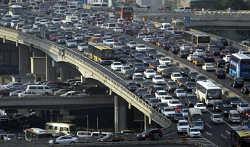
\includegraphics[width=\figwidth]{pics/17/30.png}
	\end{center}
\end{wrapfigure}
Unless you've actually been in a Hive it's impossible to truly understand how unpleasant navigating one via a ground vehicle is. 
If you want a general idea though, take the messiest, worst designed, most overloaded traffic system you've ever encountered and then make it three dimensional, fill any gaps with poisonous smog, and finally populate it with the most aggressive idiots this side of an Orkish Warband. 
Just navigating the place was a miserable experience, when you factored in our van's lack of seats, air conditioning, or proper filtration systems, it got downright hellish.

Of course hellish conditions are part of a Guardsman's job description, so we suffered through nearly two weeks of automotive torture with no more than a moderate amount of bitching. 
Day after day, we followed that damned scan-van around at a distance of "no more than six hundred and no less than four hundred meters", idly noting the way other drivers subconsciously made way for it but not us and how carjackers and other such bottom feeders always ignored the immaculate vehicle in favor of our obviously worthless van. 
Then, every night, we were summoned into the evening holo-conference with the Inquisitor to report that we'd done nothing but sit in a van all day and futilely request actual bloody seats for our vehicle. 
The requests were rejected of course, as were our ones for actual intel on what the mission was and orders that had an actual point aside from just pissing us off, and we were then kicked out of the meeting before operational security could be compromised by us overhearing the rest of team's reports or the Inquisitor's brilliant fucking deductions.

\begin{wrapfigure}{O}{\figwidth}
	\begin{center}
		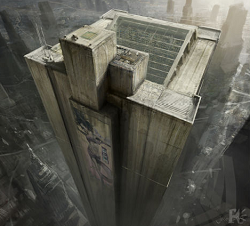
\includegraphics[width=\figwidth]{pics/17/31.png}
	\end{center}
\end{wrapfigure}
So, what amounted to our "day job" sucked. 
It was uncomfortable, stressful, and (as far as we could tell) completely pointless. 
Seriously, it wasn't like they the team was even doing any real missions, they were just sifting for data and were far better equipped to get themselves out of trouble than we were. 
Five heavily armed men opening up on an overenthusiastic carjacker, or launching an armed extraction into an up-hive fancy dress party for that matter, is the sort of thing that hostile Inquisition-types notice, and as we were repeatedly reminded by our boss, being noticed would be a BAD thing. 


Honestly, it felt like every aspect of our assignment was purposely designed to piss us off, except we were pretty sure that the Inquisitor didn't actually care enough about us to rearrange the whole mission just to spite us. 
Well, except the shittiness of the van, that had to have been his idea, or the Tech-Priest's, we decided to split the difference and just hate them both, but not as much as we hated the van itself. 


Not that our time outside of the van was any better. 
The Inquisitor had decided that we would "have to be as the sharks, swimming in the sea of humanity, moving silently, lest the ripples of our passage forewarn our prey". 
Which apparently meant that, instead of a nice securable warehouse or office complex or luxury apartment, we'd be making our base in the middle of a bloody hab block. 
Sarge had lodged a protest, citing the impossibility of properly securing a base surrounded on six sides by civvies without everyone and their mother noticing. 
This just earned him a lecture on how futile mere physical defenses were, as well as a reminder that absolutely no defensive explosives were to be used in our security measures. 
The ensuing argument about whether we'd been justified in blowing an entire floor of one of the Inquisitor's previous bases to shrapnel, along with the hostile hit squad that'd been on it, got Sarge ejected from the briefing.

\begin{wrapfigure}{O}{\figwidth}
	\begin{center}
		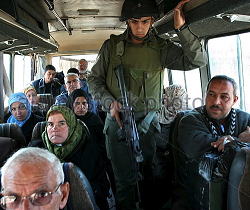
\includegraphics[width=\figwidth]{pics/17/32.png}
	\end{center}
\end{wrapfigure}
So the entire ground team wound up crammed into handful of adjacent habs halfway up a lower-middle-hive block full of manufactorum workers, Administratum scribes, and far, far too many nosy little kids. 
We secured the "half" of the base which we were assigned as best we could without a proper killing field and left the rest of the team to handle their own security.

The problem of blending in was similarly divided. 
The Inquisitor's minions procured a wide range of disguises, complete with falsified documentation inserted into the local Administratum databases and perfect local accents. 
We just tacked our old Guard insignias back on and told anyone who asked that were on leave, and threatened to shoot them if they kept asking stupid questions. 
The rest of the team claimed this was "unprofessional" and "going to get us killed along with you idiots", but failed to provide a better alternative.

Anyway, the point is that our base was cramped, insecure, surrounded by non-guardsmen, and filled with teammates that we hated more with each passing day, and despite all that, it was STILL better than driving around in that bloody van. 
Really, when you get down it, a (still-populated) Hive City is just about the worst place for a squad of guardsmen, and it was a minor miracle that we made it as long as we did before things started to fall apart.

\begin{wrapfigure}{O}{\figwidth}
	\begin{center}
		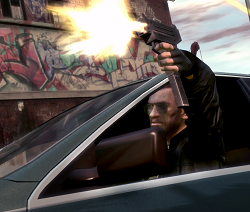
\includegraphics[width=\figwidth]{pics/17/33.png}
	\end{center}
\end{wrapfigure}
It started with Tink getting permanently relieved from driving duty due to a small incident involving a lack of merging room, an especially belligerent trucker, and Tink's oversized plasma pistol. 
Luckily, Doc was able to spoil Tink's shot, and Sarge was able to convince the traffic cops that:
\greentext{>A: There was nothing sinister about a van full of heavily armed men, because }

\greentext{>B: We were obviously just a bunch of Guardsmen on leave, and therefore }

\greentext{>C: Tink's behavior was a matter for internal Guard discipline. Have a nice day officers, here's a little something for your trouble, wink-wink, nudge-nudge, please don't tell our CO.}


So it really was just a minor incident with no significant impact on the investigation, and therefore not worth actually reporting to any of the very busy people on the other half of the team. 
Unfortunately, the police network was one of the ones being monitored by the scan-van, and the Interrogator (who was officially the ground-team leader, even though Sarge had a month or two of seniority on her bitchy ass) didn't see it that way. 


We survived the ensuing lectures without murdering any teammates, though Snitch's fun habit of loudly reporting everything we were thinking made it a close thing. 
Further flak was then earned the following evening, when after our fifth request for vehicle upgrades was rejected out of hand, we decided to pay an after-hours visit to a "recycling" shop that Nubby had spotted. 
We exchanged some second-hand Imperial Navy cabin appliances for a set of totally-not-bloodstained seats and an air-conditioning unit, and even got a sweet "Heavily Armed Buyers" discount. 
We managed to get the parts back to base without any significant problems, but only got halfway through installing the stuff before the crazy tech-priest busted in, declared our upgrades to be "an abomination in the eyes of the Omnissiah", and started ripping everything back out. 


\begin{wrapfigure}{O}{\figwidth}
	\begin{center}
		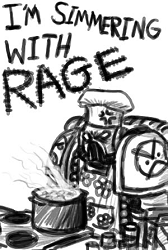
\includegraphics[width=\figwidth]{pics/17/34.png}
	\end{center}
\end{wrapfigure}
Tink and Twitch both lobbied hard for just killing the cogboy and blaming it on underhive mutants or something, but unfortunately he wasn't alone, and even more unfortunately, the man with him was Snitch, who called the rest of the team in and gleefully reported our murderous thoughts. 
Yet another painful lecture from the Interrogator followed, with our more annoying teammates chiming in to point out how useless, counterproductive, heretical, and generally incompetent we were. 
This was a bit more than even Doc and Sarge could put up with, and things devolved into a pointless shouting match that only wound down when both the upstairs and downstairs neighbors started banging on the floor/ceiling and threatening to call the police.

The rest of the night was a very tense affair, the high point being a private meeting between Sarge, the Interrogator, and the Inquisitor, which had involved a lot of yelling and detailed explanations of how unpleasant things would be for us if our "shenanigans" fouled up the mission. 
Sarge came back from that in an impressively foul mood, and was actually the one to lead us through round N+1 of the "can we get away with deserting" debate. 
Several ideas, most of which seemed to hinge on Guys that Nubby knew, were put forth, along with some rather over-the-top suggestions involving what could be left as a goodbye present for our teammates, but in the end cooler heads prevailed. 
It was agreed that, in the morning, the majority of us would go and actually apologize to the Interrogator, and see if Doc's idea to try buttering her up instead of Sciscitat would secure us some better working conditions.

Then, at around three in the morning, Twitch shot the Interrogator's dog.

\begin{wrapfigure}{O}{\figwidth}
	\begin{center}
		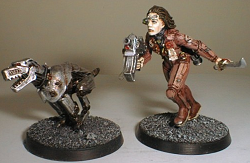
\includegraphics[width=\figwidth]{pics/17/35.png}
	\end{center}
\end{wrapfigure}
Well, it wasn't like it was actually a REAL dog, it was just Cyber-Mastiff. 
Those things have more in common with a toaster than an actual animal, and she had six of the stupid things. 
Well, five, but anyway, it wasn't like she didn't have a few to spare, and Twitch had TOLD her to stop having them patrol near our side of the perimeter. 
It wasn't that we minded having a bunch of animalistic murderous machines which only answered to a woman who hated us nosing around our quarters while we slept, no siree. 
It was just that the damned things had no sense of self preservation and would walk right into Twitch's traps unless specifically ordered not to. 
And while none of the stuff we'd been allowed to set up was lethal in and of itself, all of us had pretty violent kneejerk reactions to the sounds of a motion sensor alarm going off in the middle of the night… 

Really, it had just been a matter of time, and we'd TOLD her. 
Frequently. 
With demonstrations…

For some reason she didn't appreciate it when we pointed that out to her over the smoking remains of Cyber-Mastiff F1-D0, or whatever she'd named the stupid thing. 
Maybe it was the way Twitch kept yelling "I TOLD YOU SO".

Anyway, that was final straw. 
The Interrogator claimed it had been deliberate, Sarge told her she was being delusional, the Tech-Priest suggested having us all killed, Tink said he could fucking try, several hands started drifting towards weapons, and things might've gone very poorly if the Inquisitor hadn't chosen that exact moment to call and tell us that he'd "cracked the code".

\begin{wrapfigure}{O}{\figwidth}
	\begin{center}
		
\includegraphics[width=\figwidth]{pics/17/36.png}
	\end{center}
\end{wrapfigure}
It wasn't entirely coincidence mind you: 
a few of the Interrogator's saner teammates had decided to call a higher authority before things turned into a bloodbath. 
Sciscitat had pretty much said "that's nice, now let me tell you why I'm a genius" and commed the rest of the team so they could hear too. 
He didn't feel any need to include us in the call though, so we just had to sit there and piece together what was going on based on what we could overhear and people's responses. 


As far as we could tell the Inquisitor had found something surprising in all the data his minions had been sending him; 
so surprising, in fact, that it called for a complete change of mission objective. 
To what (and from for that matter) was a mystery to us, because Emperor forbid anyone tell the stupid guardsmen anything, but it was apparently important and time sensitive enough to push the whole shot-dog thing onto the back burner. 
Everyone started running around, and after a short whispered conversation with her boss, the Interrogator stalked away with an even grumpier than usual expression, leaving Face to relay us orders (but not any explanations). 
We decided to take what we could get, and started gearing up for action.

Three hours later, we were edging our shitty van through traffic towards some sort of lower-mid-hive office complex. 
As usual, we had absolutely no idea what was actually going on, only that Face, the Assassin, and the Interrogator would be inserting from some upper tier, and that we were supposed to park outside the 247th floor service entrance along with the scan-van. 
Given the lack of intel, we assumed that we were just there for the usual emergency backup duties, because if the Inquisitor actually wanted us to something useful he'd have at least given us a map of the building. 
At least that's what Doc had suggested, Sarge thought he was being overly optimistic, and Twitch maintained that it was all a plot by our teammates to get us messily killed.

\begin{wrapfigure}{O}{\figwidth}
	\begin{center}
		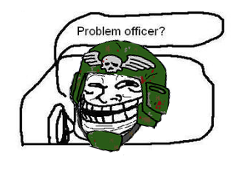
\includegraphics[width=\figwidth]{pics/17/37.png}
	\end{center}
\end{wrapfigure}
Our van, not being equipped with anti-grav or the ability to psychically influence other drivers, was the last to reach the building, and arrived just in time to watch the scan-van slide into the last available parking spot. 
After a futile search for anyone that looked ready to pull out (or bribable/threatenable), Sarge reported that we were out of position, and asked permission to either search elsewhere or dump the rest of us on the curb. 
The request was denied, the Inquisitor told the rest of the team to start the op without us, and Sarge started swearing under his breath as he reached the edge of the building and realized there was no way to turn around before crossing the skyway to the next sub-spire. 


Fifteen minutes, two highly illegal footpath-crossing U-turns, a faked engine failure, and whole lot of profanity (not to mention death-threats) from both us and other drivers, a spot was found. 
Admittedly, it was a small spot, and was labeled "Administratum Courier Vehicles Only", and was TECHNICALLY occupied, but we figured the owner of the little bike-thing wouldn't mind us relocating it to somewhere more efficient, such as the bed of the pickup truck three spots down from it. 
Nubby managed to back our three meter wide van into the two-and-a-half meter wide spot with only minor damage to the vehicles on either side, and Sarge triumphantly informed Sciscitat that we were in position. 


While the Inquisitor made sarcastic comments about how long it had taken, we checked our comms, readied our weapons, and all suffered minor heart attacks as what sounded like a small battering ram slammed into the van's rear door. 
Sarge swore and thanked the Emperor for weapons safeties as the blow was followed up by two more and a bellowed order to come out our face the wrath of the Jack Hive Traffic Authority. 
He took a breath, mustered the coolest face possible while wearing a guard-issue helmet, and cracked open the van's rear door.

\greentext{>"Problem Officer?"}


\begin{wrapfigure}{O}{\figwidth}
	\begin{center}
		
\includegraphics[width=\figwidth]{pics/17/38.png}
	\end{center}
\end{wrapfigure}
Deep in the bowels of the Inquisitorial headquarters on Holy Terra, there is an archive maintained by the Scribes of the Ordos Scriptus. 
In this archive, the most heroic victories, valiant defeats, and horrible sacrifices made by the agents of the Inquisition are recorded, so that even if the Imperium it protects may never learn of them, the greatest moments in Inquisitorial history are not forgotten. 
Our argument about Hive Parking Regulations with the traffic officer, a mere dozen meters from where our teammates were engaged in a covert operation vital to the stability of the Imperium, was not one of those moments.

It wasn't like we had any other options though: 
there were no other spots, leaving our post mid-mission would never fly with the Inquisitor, and as attractive as the idea of just shooting the man was, we were pretty sure that publicly gunning down a police officer would be considered "blowing our cover". 
So, violence and retreat not being options, we fell back on our wits, words, and Sarge's charming demeanor. 
Needless to say, it went poorly.

Now, just to be clear, Sarge's diplomatic abilities weren't the problem. 
In fact he did far better than any of us had expected, which is to say that he made it through the whole ordeal without accidentally confessing to any major crimes, revealing our mission, or assaulting the man. 
The Diplomacy Adept would've been proud. 
Anyway, the problem was that this traffic officer was the most relentless, pedantic, self-righteous bastard we'd ever encountered (which is really saying something when you work for the Inquisition). 
The man just stood there, completely implacable in his enforcement of Jack Hive Traffic Ordinances, picking apart every excuse, ignoring every appeal, and dispensing a near endless stream of tickets from his servo-skull assistant.

\begin{wrapfigure}{O}{\figwidth}
	\begin{center}
		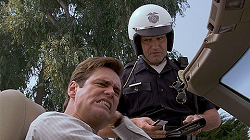
\includegraphics[width=\figwidth]{pics/17/39.png}
	\end{center}
\end{wrapfigure}
Sarge suffered through twenty minutes of that hell. 
Not out of any sort of idiotic stubbornness, but because every time he tried to shut up and take his ticket the Officer reached for his comm to call a tow vehicle. 
It was a simple choice between abandoning his post or keeping the argument going, so Sarge did his duty and repeatedly crammed his foot into his mouth. 
Well, not literally, he was just sort of hanging out of the smallest possible crack in the van's rear doors, desperately trying to hide the fact that he and everyone else in the vehicle were carrying highly illegal weapons, while he babbled for time. 
But figuratively, well, by the end he was practically shitting toes.

Of course, the rest of us didn't WANT to leave Sarge out to hang, but violence wasn't an option and it was all we were good at. 
Nubby did volunteer to trade places with Sarge, but that was shot down for obvious reasons. 
Twitch and Tink also made some suggestions that involved sneaking out and creating a distraction, unfortunately the only door that wasn't wedged close by the surrounding vehicles was the one Sarge occupied, and busting out the windshield didn't seem very sneaky. 
Doc's more practical idea to call for help from our team, or at least get permission to fall back, didn't work out any better. 
Whether they were actually busy, or were just being asses were unclear, but our teammates in the scan-van claimed they had better things to do then help us get out of a parking ticket, and the Inquisitor just told Doc to get off the shared comm channel. 
In retrospect he probably should have described the problem as a potential hostile agent, or an Arbite, or anything other than a traffic cop really.

\begin{wrapfigure}{O}{\figwidth}
	\begin{center}
		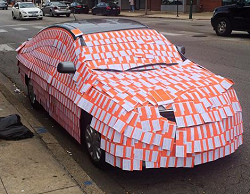
\includegraphics[width=\figwidth]{pics/17/40.png}
	\end{center}
\end{wrapfigure}
So lacking anything useful to do, the rest of us just sat there, listening to the rest of team's comm chatter and praying to the Emperor that one of them would screw up, and the death of Imperium's most annoying Traffic Officer could be put down as acceptable collateral damage. 
That didn't happen though, which was probably a good thing given how important the information our teammates extracted turned out to be… 

Anyway, by the time word finally came down that the objective had been completed and it was time to pull out, Sarge's twenty minute argument with the Officer netted us citations for:
\greentext{>Parking in a Restricted Area}

\greentext{>Failing to Vacate in a Timely Manner}

\greentext{>Operating a Commercial Vehicle Without a Permit}

\greentext{>Impersonating a Commercial Vehicle}

\greentext{>Failing to Vacate in a Timely Manner}

\greentext{>Operating an Administratum Courier Without a Permit}

\greentext{>Impersonating an Administratum Courier Vehicle}

\greentext{>Failing to Vacate in a Timely Manner}

\greentext{>Tampering with an Administratum Courier Vehicle}

\greentext{>Loading or Unloading a Vehicle in a No-Loading Zone}

\greentext{>Failing to Vacate in a Timely Manner}

\greentext{>Attempting to Bribe a Traffic Officer}

\greentext{>Attempting to Threaten a Traffic Officer}

and
\greentext{>Failing to Vacate in a Timely Manner}


The whole thing was thoroughly humiliating, ended with a total fine of over twelve-hundred thrones as well as three separate court summons, and since we were never actually called on to do anything, was completely pointless. 
That said though, we managed to maintain our position without actually being arrested or starting a shooting war with the local authorities (though admittedly things got pretty close near the end there), so we were willing to call it a moral victory. 
Mind you, the Inquisitor and his minions didn't see it that way, but fortunately they were a little too caught up discussing the data they'd extracted to do more than make a few sarcastic comments.

\begin{wrapfigure}{O}{\figwidth}
	\begin{center}
		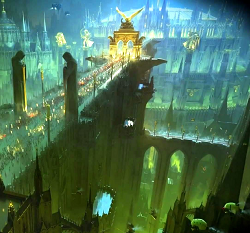
\includegraphics[width=\figwidth]{pics/17/41.png}
	\end{center}
\end{wrapfigure}
By the time we finally escaped the Avatar of Traffic Ordinances (the second he'd realized Sarge was pulling out, all that "vacating in a timely manner" stuff had gone out the window and the bastard had started dragging his feet with a sort of grim vindictive glee), the rest of the team had finished pulling out, held one of their no-guardsmen-allowed meetings, determined that SOMEONE was SOMEWHERE, and had all started heading off towards some place in the upper hive. 
We knew this because every five minutes or so the Inquisitor commed us to ask why we hadn't left yet; 
Sarge wisely removed his combead and put Doc in charge of talking to the man.

It took us three hours of driving to climb above the smog layer, through the middle levels, and into the relatively low section of the upper-hive where whoever we were chasing was. 
This was longer than the Inquisitor wanted it to take, but it at least gave Sarge some time to calm down, and after the first hour we were able to ditch the rebreathers, so it was actually relatively pleasant. 
In fact we made it the whole way without encountering any serious traffic problems, or even seeing a single cop, which was great for both our nerves and their continued survival, but probably should have stuck us as a little odd. 


Anyway, everything was uneventful and relaxing right up until we were about two kilometers from our destination, which turned out to be a chapel dedicated to some local Saint. 
It wasn't the largest place, at least by hive standards, but whoever "Castor the Obviate" was, the locals at least thought he rated his own sub-spire, with a shuttle port and road connection to boot. 
We were in the middle of trying to figure out how best to get to said skyway from our exit when the mission's timetable abruptly accelerated.

\begin{wrapfigure}{O}{\figwidth}
	\begin{center}
		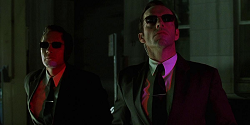
\includegraphics[width=\figwidth]{pics/17/42.png}
	\end{center}
\end{wrapfigure}
From what we'd overheard on the comms, our teammates were more or less in position to launch an infiltration of the Ecclesiarchy-only sections of the chapel. 
As usual, we had absolutely no idea WHY they were doing this, only that it involved some guy who was hiding there. 
Who he was, what he looked like, and whether the end goal was to kidnap, interrogate, kill, or bake a cake for the sucker was completely unclear.; 
apparently it wasn't something we "needed to know". 
The same went for what OUR whole role in this operation was and why in the Emperor's name they were delaying everything to wait for us, but that turned out to be a moot point since the mission went off the rails before we even got there.

Everyone but us was more or less in position. 
The scan-van was parked outside, Face and the Interrogator were already inside one of the chapel's public areas, the Cleric was chatting up a fellow fanatic near a service entrance, and the Assassin was being all assassiny on the roof. 
Then the Tech-Priest noticed a sudden increase in encrypted vox traffic and Snitch sensed several hostile minds entering the area. 
This was followed by Face announcing that a pair of local Secret Police-types moving towards the target, the Cleric and Assassin reporting that their entrances were now blocked, and the Interrogator loudly blaming all of it all on us for taking so long to get there. 
Tink responded by pointing out that WE hadn't asked them to wait for us, and followed it up with some choice comments about her personality and parentage, which she reciprocated. 
Sarge made a half-hearted attempt to shut Tink up, but was beat to it by the Inquisitor, who cut both their comms and started belting out an impressive stream of orders, of which ours were "get into position right now, or by the Emperor I will make sure you incompetents die before I do".

\begin{wrapfigure}{O}{\figwidth}
	\begin{center}
		
\includegraphics[width=\figwidth]{pics/17/43.png}
	\end{center}
\end{wrapfigure}
As tempting as it was to take our damned time, there's nothing quite like an Inquisitor issuing orders in a tone of suppressed terror to motivate a cooperative attitude. 
Nubby (who's lack of scruples made up for his innability to see all the way over the dashboard, and was already in the seat in any case) put the metal to the pedal to the other metal, and started weaving through traffic like he had a Tau hover-tank on his ass while Sarge navigated. 
Speed limits and lane markers were ignored, signs and lights were treated as amusing suggestions, and anything smaller than us was trusted to look out for itself (or in the case of one of those Administratum couriers, wind up clinging to our hood and screaming in a most unhelpful manner until Sarge pried them off).

Between our obvious willing to trade hits, superior guardsmanly reflexes, and a whole lot of luck, we made it to the skyway in under five minutes, only to discover that the road to the chapel was at a complete standstill. 
Sarge eyed the jammed lane leading to the chapel, then the nearly empty lane leading FROM it, and told Nubby to go for it. 
The rest of us gripped onto whatever surfaces we could find, and prayed to the Emperor that everyone on the bridge was more chicken than us.

Fifty-four heart-stopping seconds and three near misses later, our shitty van screeched around the Secret Police vehicle that was in the process of cordoning off the outgoing lane (nearly crushing the officer in the process), jumped a section of sidewalk, and power-slid into the last available spot in front of the Chapel's main entrance. 
Nubby killed the engine with a half-hysterical giggle, Tink helped pull Twitch out from where he'd gotten wedged, and Doc reported our position to the Inquisitor.

Sarge slumped back in his seat with a sigh of relief, only to jerk upright as an armored glove slammed against his window, and a horribly familiar growl of a voice asked him if he knew how many traffic laws he'd just violated.

\begin{wrapfigure}{O}{\figwidth}
	\begin{center}
		
\includegraphics[width=\figwidth]{pics/17/44.png}
	\end{center}
\end{wrapfigure}
The expression on Sarge's face… well, let's just say he managed to sink his fingers about a centimeter into the dash during the few seconds it took us to rig up a camo tarp to hide the rear of the van from sight. 
Fortunately, by the time we'd finished and he rolled his window down, he'd regained enough control to limit himself to merely glaring at the Officer in an attempt to kill the man via pure concentrated hatred.

As Sarge announced that no, he did not know how many laws he'd broken, but would appreciate being informed, in detail, by the helpful officer, the rest of us quietly argued about what the hell was going on. 
It was fairly obvious that the Officer had followed us on his hoverbike, but why was less clear. 
A properly paranoid Inquisitorial team would've probably assumed he was purposely trying to interfere with our mission (in fact, that's exactly what our teammates said when Doc told them), but we were less sure.

For one thing, if the Officer was some sort of enemy agent, or their catspaw, he should've actually LOOKED like a normal cop. 
His kit was perfectly regulation, and there really isn't any rule that says a traffic cop can't be a two meter, hundred twenty kilo mountain of muscle…  But your average traffic cop doesn't practically vibrate with the internal anger of an officer who wants nothing more than to arrest the entire planet, from the lowliest underhive grubber to the Planetary Governor, for not doing it right. 


Then there was the way the actual agent types on the scene reacted. 
As Sarge began arguing his way into another massive pile of tickets, a pair of those planetary secret police guys (possibly the ones who'd been setting up the roadblock we'd bulled through) came running up, only to freeze in their tracks as they sighted the Officer. 
After a brief argument, the two of them had lowered their weapons, carefully backed away, and very pointedly went to find something else that needed their attention. 
Very interesting that.

\begin{wrapfigure}{O}{\figwidth}
	\begin{center}
		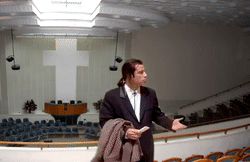
\includegraphics[width=\figwidth]{pics/17/45.png}
	\end{center}
\end{wrapfigure}
Or to put it all another way, we'd been in the Inquisition long enough to recognize a monomaniacal fanatic when we were issued a parking ticket by one. 
Doc, being the current comms bitch, reported our reclassification of the Officer from "threat" to "very annoying hazard" to the Inquisitor, who responded by yelling at him for kicking up a fuss about it in the first place. 
Doc took this with good grace, because from the sound things it probably wasn't the best time to get snippy.

Based on what we could overhear on the general channel and see though the rust-holes in our van, things weren't going too smoothly for our teammates. 
There was a lot of chatter about diverting the Secret Police and the target having run off, the Assassin kept asking for directions through air vents, the Cleric needed someone to open a door, and the scan-van was relaying all sorts of worrying info about incoming reinforcements. 
Things certainly didn't sound good, but they hadn't degraded to the point where they wanted us involved either, so we just sat in our van like good little guardsmen and waited for our orders. 
Lacking anything else to do, most of us were engaged in Twitch's sixth and seventh-favorite pastimes of tracking potential hostiles and planning preemptive strikes, when Sarge stuck his head around the tarp and announced that he needed two volunteers to run a quick errand.

Volunteers in this case meaning whoever looked the least likely to get themselves arrested the second they stepped out of the van. 
Since Twitch currently had pin-less krak grenades in both hands, and Tink had his goggles on and was resting the tip of his oversized plasma-pistol against the section of paneling between him and the Traffic Officer, the options were limited. 
Five minutes later Doc and Nubby were standing at the top of the chapel's stairs, avoiding eye contact with Secret Police officers and trying to figure out just where in that most holy shrine one could get one's parking validated.

\begin{wrapfigure}{O}{\figwidth}
	\begin{center}
		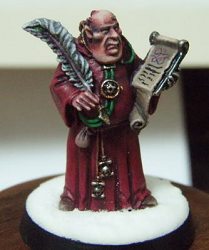
\includegraphics[width=\figwidth]{pics/17/46.png}
	\end{center}
\end{wrapfigure}
The Officer hadn't even blinked when two men in full guard-issue carapace armor (with helmets) climbed out of the van, though he did issue Sarge a ticket for being over his vehicle's rated passenger capacity. 
The crowd of up-hive pilgrims inside the Chapel foyer didn't seem to care much either, being rather more focused on their prayers or all the Secret Police running around. 
As for the Secret Police, after a cursory glance revealed that Doc and Nubby weren't carrying any weapons, they were just ignored with that special flavor of disdain that "elite" units seem to reserve for those of us who do the real work. 
Our teammates on the other hand, immediately started complaining over the comms about us being out of position and blowing our cover. 
Doc responded by asking if THEY knew where the parking validation guy was, but didn't get an answer.

Doc and Nubby's wandering search for the Holy Secretary of Parking Validation was brought to an abrupt end by a shout of "HE'S GETTING AWAY" from the Interrogator, and a potbellied man in scribe's robes bolting into the foyer from corridor. 
A quick glance revealed a group of Ecclesiarchy guards following the man, and a pair of Secret Police moving to cut him off from the main doors with Face hard on their heels. 
Doc and Nubby shared a glance then split up: 
Doc weaving through the crowd towards the Ecclesiarchy guards, and Nubby sidling towards the Chapel entrance.

\begin{wrapfigure}{O}{\figwidth}
	\begin{center}
		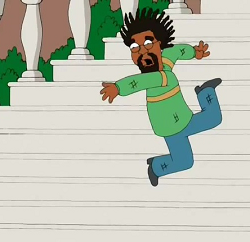
\includegraphics[width=\figwidth]{pics/17/47.png}
	\end{center}
\end{wrapfigure}
If the sprinting scribe had been paying any attention, he might have noticed a confused-looking guardsman holding a parking ticket abruptly stepping out into the path of his pursuers, mirroring the lead-guard's dodge, and taking the whole group out in a pile of tangled limbs. 
Or if he'd been looking to his left, he could've seen a random pilgrim pull a similar maneuver, tripping up two Secret Police officers but not the man following them. 
The scribe didn't see either of these crashes though, in fact he was so focused that he didn't even notice when an ugly little man near the Chapel doors stuck out an augmetic leg. 
Well, at least not until his shin-bone, weakened by years of malnutrition and pollution-induced illness, shattered like a stick of chalk.

As the scribe tumbled forwards, grasping for his leg instead of reaching out to break his fall, Nubby's grubby little hands missed the man's upper arm entirely, settling on one of the augmetic cables coming out of his head instead. 
The short trooper's powerful backward lunge, intended to spin a significantly larger man off to the side and out of sight of pursuers, ripped the cable right out the Scribe's skull, and launched both it and Nubby a full two meters into the air. 
On the plus side, this gave him an excellent view as the Scribe tumbled through the Chapel's doors, slid across the polished marble landing, and sailed right over the edge of stairs.

Sarge and the Traffic Officer both turned to watch as a screaming figure in scribe's robes crashed down seven flights of stairs, scattering pilgrims and finally crashing in a twitching, bleeding heap directly in front of the Officer who, after a second's consideration, issued the man a ticket for obstructing a public walkway.

Nubby's embarrassed "Oops" echoed for a second over the dead silence comm channel, then the yelling started.

\begin{wrapfigure}{O}{\figwidth}
	\begin{center}
		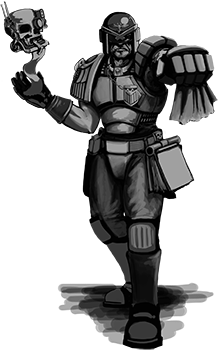
\includegraphics[width=\figwidth]{pics/17/48.png}
	\end{center}
\end{wrapfigure}
Left to his own devices Sarge would have been hard pressed to decide whether to laugh, cry, or dash up the stairs to strangle Nubby with his bare hands, but he only had a limited amount of time and the Inquisitor was issuing some very sub-optimal orders.

Sciscitat wanted us to throw the nearly-dead Scribe into our van and run for it, but Sarge had eyes on at least a dozen heavily armed Secret Police, and was very aware of the differences between our shitty van and an APC. 
The only reason said Secret Police weren't already moving in was the presence of Traffic Officer. 
The huge cop wasn't actually doing anything to protect, or even help, the Scribe, but when the first Secret Police agent showed up, the Officer turned a glare of such concentrated hatred on the man that he actually fell over in his haste to back up. 
A sort of standoff had developed, with the Officer standing completely still in the middle of a sevenish-meter ring of curious onlookers and obviously terrified Secret Police. 
Sarge put the question of just what the hell was going on with THAT out of his mind, and seized his chance while the Officer was distracted to relay an "interpreted" version of the Inquisitor's orders to the rest of us. 


Operating on the theory that what the Inquisitor actually wanted was a chance to brain-scan the Scribe before the Secret Police got to him, Sarge decided that what we'd actually been told to do was "secure" the man. 
The fact that the Officer's goon-repelling aura was already doing this without any effort on our part was just a happy coincidence. 
Of course, this still left the problem of getting the actual brain-scanning done without the Secret Police noticing, not to mention keeping the nearly-dead Scribe alive long enough for it to happen.

\begin{wrapfigure}{O}{\figwidth}
	\begin{center}
		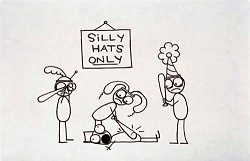
\includegraphics[width=\figwidth]{pics/17/49.png}
	\end{center}
\end{wrapfigure}
Less stalwart and dutiful men might've decided it wasn't their problem and dumped the whole brain-scanning problem on teammates and superiors, but we were above that sort of thing. 
Honestly.

Okay, well, maybe not... 
but we WERE pretty sure that any requests for assistance would result in more orders to get ourselves shot doing something stupid, which is why we decided to just go ahead with our own little plan before anyone had a chance to tell us not to. 


Step one of said plan consisted of Twitch and Tink bailing out of the van while everyone was distracted. 
Tink jogged up to the Chapel to retrieve Doc, who had just finished getting the shit kicked out of him by the three Chapel Guards he'd tripped up. 
Of course, since he'd been wearing his armor, the beatdown mostly just resulted in a few broken toes for the kickers, but the medic was still a bit woozy when Tink pried him off the floor. 
Doc successfully collected, the two of them headed back out of the Chapel, carefully avoiding the area where Nubby was deflecting any suspicion by loudly complaining about how he (a "poor ol' vet'ran wat 'ad 'is legs blown off in da war") had been struck by some crazy running person, and demanding some sort of reparation from the Chapel. 
Preferably cash.

While Doc was being retrieved, Twitch made his way over to where the Scan-Van was parked and asked if Snitch could step outside for a minute. 
The psyker and Tech-Priest tried to ignore him at first, but Twitch being Twitch, that proved to be rather difficult. 
The demolitions trooper, who hated crowds, exposed positions, and being anywhere near armed hostiles to start with, and was even less happy about leaving his lasgun and most of his explosives in the van, wasn't in the mood for silly little games and made that abundantly clear. 
There's just something about a man on the very edge of a psychotic breakdown banging on your door with a live anti-tank grenade that's impossible to ignore.

\begin{wrapfigure}{O}{\figwidth}
	\begin{center}
		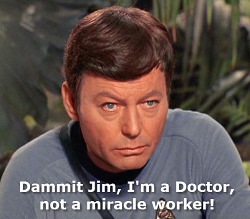
\includegraphics[width=\figwidth]{pics/17/50.png}
	\end{center}
\end{wrapfigure}
Back at our van, the standoff between the Officer and the Secret Police gradually intensified as more and more of them arrived and the Scribe's condition steadily worsened. 
Sarge, being very familiar with the look of men trying to psych themselves up for a possibly-fatal attack, waited until it looked like the Secret Police were just about to find their spines before stepping in.

Right as the tension reached the breaking point, Sarge opened his door, walked up behind the Officer, and in his best noncom shout, asked just what in the Emperor's name was going on here. 
Even expecting it, Sarge only barely ducked the reflexive haymaker from the startled Officer, but continued his obviously-rehearsed speech without missing a beat. 
Putting on a show of surprise that wouldn't have fooled the most gullible toddler, Sarge pointed to the mangled Scribe and asked what had happened. 
After a short pause for someone to start answering, Sarge interrupted to point out that the man obviously needed a medicae, asked why one hadn't been called, waited again, and then interrupted THAT answer with a bellow of "MEDIC". 
Right on cue, Tink shoved a confused and winded Doc out of the crowd.

The medic stood there for a second, taking in the full extent of the Scribe's injuries and automatically reached for his concealed sidearm instead of his medkit. 
He was brought up short by a grunt from Sarge. 
There was an awkward moment as Doc gave Sarge a "you've got to be kidding" look and Sarge tried to convey "start treating this poor bastard before we're all shot" via more grunts and a few head jerks. 
After a few seconds of this Tink realized that Doc's combead must have been damaged during his beatdown and the medic had absolutely no idea what was going on. 
Lacking any better ideas, Tink just yelled at Doc to stop standing around and get to work, which entirely failed to convey all the nuances of our plan, but at least it got the medic moving.

\begin{wrapfigure}{O}{\figwidth}
	\begin{center}
		\includegraphics[width=\figwidth]{pics/17/51.png}
	\end{center}
\end{wrapfigure}
Whatever the Officer or the Secret Police thought of the whole charade, neither group seemed willing to intervene as Doc gave the Scribe emergency stimulants, transfusions, and more-icky varieties of first-aid. 
This might've been because our amazing acting skills had taken them all in, but it probably had more to do with the fact that Doc's efforts were so obviously futile. 
Seriously, the man's shinbones were coming out his armpits; 
he looked like a cross between a pretzel and a pancake, except with a lot more blood. 
The only thing keeping the Scribe alive was a metal skull and a few augmetic internal organs which were already in the process of failing.

Of course, once Doc got going, he was the best show in town: 
there's something horribly fascinating about watching someone trying (and generally failing) to put a human jigsaw puzzle back together. 
None of the Secret Police even noticed as Twitch more or less dragged Snitch through the crowd and up to the edge of the circle around Doc and his patient. 
Not that they would've objected if they had noticed, nothing unusual about yet another guardsman and an average-looking pilgrim trying to get a better view. 
The tricky part of was going to be getting the annoying psyker the last few meters and making sure nobody noticed anything warpy. 


Fortunately, by the time Snitch was in position, Doc had been brought up to speed. 
Not by Sarge mind you, after a few increasingly comical attempts to grunt instructions at the Medic, the Traffic Officer ordered him to get back into the van or be arrested on the spot. 
Tink on the other hand, decided to check whether Doc's combead was really broken or had just gotten switched to another channel during his beatdown. 
The fact that the channel it'd been switched to turned out the be the one shared with the rest of the team was a bit inconvenient, but most of them were too busy trying to steal something or other without getting shot to do more than call our plan dangerously stupid.

\begin{wrapfigure}{O}{\figwidth}
	\begin{center}
		\includegraphics[width=\figwidth]{pics/17/52.png}
	\end{center}
\end{wrapfigure}
As soon as he saw Snitch, Doc announced in the voice of medical authority that he needed three volunteers to help with his patient, specifically Snitch, Twitch, and (just for appearances) the queasiest looking Secret Policeman he could see. 
Snitch was told to immobilize the Scribe's head, Twitch was ordered to remove what was left of the Scribe's robes, the Secret Policeman (who was practically quivering under the full force of the Traffic Officer's glare) was just handed a big handful of miscellaneous organs to "hold on to". 
He immediately dropped the liver.

Now, on the big list of cunning Inquisitorial gambits, just brain-scanning the guy right in front of two-dozen hostile agents and hoping really hard they wouldn't notice, probably places somewhere near the bottom. 
Afterwards our teammates (Snitch especially) were all too happy to point out the numerous things that could've gone wrong and what that would've meant for their super important secret mission thing. 
That said though, we pulled it off without a hitch. 
Well, mostly. 


Snitch managed to do his thing without accidentally tearing a hole in reality, but the Scribe finally kicked the bucket about halfway through. 
When this happened Snitch began whispering over the shared channel about a copy of the data being stored on some sort of device the Scribe was carrying. 
Twitch began rooting through the wad of bloody clothes he'd ripped of the man, but suddenly found himself looking up the Traffic Officer's shock-maul and being informed of that any further rummaging would constitute a class-7 violation. 
This in turn, caught the attention of the Secret Policeman, who suddenly remembered what his actual job was and tried to take the wad of clothes from Twitch without dropping any of the organs he was still holding. 
Twitch refused to let go, and an awkward tug-of-war began, with neither side willing to actually do anything overt enough to catch the Traffic Officer's attention.

\begin{wrapfigure}{O}{\figwidth}
	\begin{center}
		\includegraphics[width=\figwidth]{pics/17/53.png}
	\end{center}
\end{wrapfigure}
While Twitch and the Secret Policeman struggled over the Scribe's clothes, Doc decided to check if any of the dead man's augmetics were the data-storage device. 
This proved to be a bit tricky, since neither he or Snitch knew what the device looked like, and they both had to maintain the fiction that the Scribe was still alive and their rummaging was just an especially invasive method of treatment. 
After a few minutes of this nothing had been turned up, the Secret Police around us were getting visibly antsy, and Snitch was making "I really should get back to my armored scan-van before these guys shoot me along with you idiots" noises. 


As the tension mounted Doc and Twitch tried to make one last attempt to determine whether the data was in the Scribe's body or clothes, Tink circled back to van to grab everyone's weapons, Sarge quietly argued with the Inquisitor over whether to run or fight, and Nubby asked if the "fingy" looked anything like a dataslate connected to a neural interface cable. 
Because he might've, y'know, accidentally sort of found something like that. 
Just now, lying on the ground, completely new development, certainly not something that had been sitting in his pocket for the last fifteen minutes.

Within twenty seconds of Nubby's question over the general channel, the augmetic dataslate thingy had been seized by Face and plugged into one of the Inquisitor's data-collector devices. 
Before the upload had even finished Sciscitat announced that it was the information he'd been looking for, and ordered his minions to pull out and "leave the Ministorium their copy". 
He also went on for a bit about him being much smarter than someone or other, and how a head start was more than enough of an advantage for someone of his genius, but we were a little busy trying to get the hell out of there to pay much attention to him.

\begin{wrapfigure}{O}{\figwidth}
	\begin{center}
		\includegraphics[width=\figwidth]{pics/17/54.png}
	\end{center}
\end{wrapfigure}
Our evac was a fairly orderly one. 
At Sarge's order over the comms, Twitch abruptly gave up in the tug-of-war over the Scribe's robes with the Secret Policeman, who immediately toppled backwards over the remains of the Scribe. 
As the man picked himself back up, Doc announced that his patient was "stable" (it being hard get much more stable than dead), and asked the Secret Policeman if he could provide a vehicle to transport the Scribe to the nearest hospital. 
After a glance at the Traffic Officer, who didn't say anything to veto this, the Secret Policeman accepted and called for a hovervan.

What was left of the Scribe was peeled off the pavement and loaded into the back of the Secret Police van without incident, though the Traffic Officer did issue the vehicle tickets for parking on the sidewalk, loading/unloading in a non-designated area, and operating without plates or registration. 
None of the Secret Police seemed inclined to dispute these tickets, and the second the Scribe was loaded the whole lot of them just sort of melted back into the crowd and disappeared. 
After a few seconds of hesitation, Snitch scampered off as well, leaving just us and the Traffic Officer, who immediately asked Doc for the validated parking pass.

Doc's second quest to find the parking validation office went a bit better than the first one, largely thanks to the fact that Nubby had already talked to the Chapel administrator in charge of it as part of his injured-veteran routine. 
The poor woman was willing to do pretty much anything to get him out of the place faster, and even threw in a few vials of holy water plus a coupon for a free blessing at some shrine on the opposite side of the planet. 
Our parking validated, Sarge collected our massive sheaf of tickets, and we drove our shitty van back into Jack Hive proper with the Traffic Officer very obviously following us on his hoverbike.

\begin{wrapfigure}{O}{\figwidth}
	\begin{center}
		\includegraphics[width=\figwidth]{pics/17/55.png}
	\end{center}
\end{wrapfigure}
It took us nine hours to lose the Traffic Officer. 
NINE. 
The Inquisitor and his minions had time to go back to our base, analyze their precious data (which we certainly weren't thanked for providing), plan the next mission, and even scout out the target location, all while we played cat and mouse with that relentless bastard. 
We went through just about every trick imaginable, even bribing other vehicles to violate laws in an attempt to draw him off, he just ignored it all and kept riding our ass like some sort of unstoppable traffic-oriented angel of vengeance. 
After five hours we were ready to throw in the towel, but the Inquisitor wouldn't let us: 
he was all like "blah blah operational security blah blah might be a Conspiracy agent blah blah", and forbid us from going anywhere near the base until we shook him.

The best part of the whole ordeal was the complete lack of support from our team. 
For all his talk about the Officer being this big threat to security, the most he was actually willing to do to help us was send the man's public record to Tink. 
While this was completely useless to us, it did at least explain that the reason the man looked like an Arbite crammed into a traffic cop uniform was that he WAS one. 


Specifically he was the official Arbites liaison to the Jack Hive Traffic Patrol, which accounted for his general interest in traffic if not why he was out issuing tickets and harassing honest guardsmen instead of liaising. 
Aside from that, all the file said was that he'd been liaising for about a year, had been in the Arbites proper for over fifty, and held the rank of Trooper. 
This seemed odd, especially since Tink had heard at least one Secret Policeman refer to him as "The Judge", but the rest of his record was classified and the Inquisitor claimed that hacking into the Abites databases wasn't worth the risk. 
Further requests for information and assistance from our team resulted in variations of "we're busy, deal with your own shit".

\begin{wrapfigure}{O}{\figwidth}
	\begin{center}
		\includegraphics[width=\figwidth]{pics/17/56.png}
	\end{center}
\end{wrapfigure}
Anyway, long story short, we had what looked like a disgraced Arbite following us, and the only way we managed to shake him was by driving through an active underhive gang-war. 
Seriously, that's what it took, it was either that or shoot him ourselves, and as attractive as that sounded, we were pretty sure there was a reason those Secret Police hadn't been willing to try it.

So yeah, gang war. 
It was at about the seven hour mark when Twitch came up with the idea, and by that point we were all so tired of trying to nap in the back of the van that we just went with it. 
We cruised around the lowest drivable regions of the hive until Tink picked up chatter about a serious gunfight, and then we just drove right through the middle of it. 
Repeatedly.

Yes we got shot at, and yes they hit the van a few times, but they were mostly using cheap autoguns and carapace armor is pretty sturdy stuff, so the worst of the damage was the windshield and Doc's recaff mug. 
That was all just casual potshots and stray bullets though, the Officer on the other hand might as well have had a giant neon bullseye painted on his bike. 
In his defense, he was probably used to going around in Arbite gear, which tends to both be sturdier and protected by their penchant for disproportionate responses. 
After the second lap he was barely staying in the air, and halfway through the third someone nailed his forward anti-grav thingy with a hand-cannon. 
We watched him go down and saw what looked like a bunch of kids armed with pipes swarm the landing site. 
We decided that that was probably as good as we were going to get and cheesed it.

We re-emerged into the more lawful levels of the hive drunk with victory and on the lookout for a good breakfast opportunity. 
Unfortunately the second we got back into clear comm contact with the Inquisitor he started yelling at us to head towards the next mission. 
So Arbite-less, but also pancake-less, we headed towards the bank our teammates were planning to rob.
Previous Chapter: